\chapter{Vector Spaces}

Words of Advice to Mathematical Scientists:\\
\begin{center}
    {\bf LINEAR ALGEBRA IS THE MOST IMPORANT OF ALL OF THE MATHEMATICAL SCIENCES}
\end{center}
Why?
\begin{itemize}
    \item Within linear algebra is the language that describes all of the how and why
        for all linear operations.
        \begin{itemize}
            \item solving linear differential equations
            \item the reasons why the derivative and the integral operators work so nicely
            \item geometry and transformations
            \item computer graphics (video games are 99\% linear algebra)
            \item image processing (Photoshop = fancy linear algebra package)
            \item large scale stress computations (linear elasticity)
            \item \dots
        \end{itemize}
    \item Linear Algebra is {\bf far} more than just {\it matrices}.
\end{itemize}

\section{What is a Vector Space}

To get properly in to Linear Algebra we first need to establish some of the common
notation.  You are familiar with 2D and 3D Vectors but using the spatial notion of
``dimension'' limits how you will think about vectors in linear algebra.  Instead of
thinking of the spatial dimensions that we live in you should be thinking of vectors as
abstract objects with mathematical properties.  Your intuitive notion of ``arrows'' is
limiting and ultimately incorrect for many purposes.  This chapter starts us in the direction of abstract
vector spaces, but don't be worried that we will be doing abstract mathematics.  We are
not abstracting a familiar notion for no good reason.  It was this very abstraction that
has allowed mathematics to advance over the past several centuries.

Let's briefly talk about how you learned about functions.  First you were told to think of
a function as a ``rule'' that accepted an input and gave a single output (high school
algebra).  Then you got used to the notion that you could add, subtract, multiply, and
divide functions to get new functions (pre-calculus).  When you took calculus you started
to think of functions as {\it objects} themselves and started discussing ways to get
properties of those objects.  The process that you've gone through with functions is
called ``objectification'' of a mathematical idea: you have turned functions into objects
in your mind's eye.  Our goal in this chapter is to ``objectify'' the idea of vectors.  We
are going to turn them into abstract objects that have mathematical properties.



\begin{definition}[The Spaces $\mathbb{R}^n$]
    Some common vector spaces (and common mathematical notation)
    \begin{flalign*}
        \mathbb{R}^2&= \{ (x,y) \, : \, x,y \in \mathbb{R} \} \\
        \mathbb{R}^3&= \{ (x,y,z) \, : \, x,y,z \in \mathbb{R} \} \\
        \mathbb{R}^4&= \{ (x_1,x_2,x_3,x_4) \, : \, x_j \in \mathbb{R} \quad \text{for}
        \quad j \in \{1,2,3,4\} \} \\
        \vdots\\
        \mathbb{R}^n&= \{ (x_1,x_2,\ldots,x_n) \, : \, x_j \in \mathbb{R}  \quad \text{for}
        \quad j \in \{1,2,\ldots,n\}\} 
    \end{flalign*}
\end{definition}
\begin{problem}
        ($<5$ minutes): Make a list of all of the things that you can do to vectors in $\mathbb{R}^2$ and
        $\mathbb{R}^3$ and give examples of how you do them.
\end{problem}
\solution{
Students likely list addition, subtraction, scalar multiplication, maybe the cross product
(but this doesn't have a great meaning above 3D), projections, length, zero, etc.
}

The list that you made for vectors in $\mathbb{R}^n$ is really just a wish list of all of
the things that you would like out of a well defined collection of mathematical objects
called ``vectors''.  We are going to abstract the idea so that we do not have to just
think about arrows and lines in space.  Instead, a {\it vector space} is a collection of
abstract mathematical objects that satisfies a collection of rules (the rules that you
likely already wrote down).


\begin{definition}[Vector Space]\label{defn:vs}
    A {\bf Vector Space} $\mathcal{V}$ is defined as a set of {\it mathematical objects}
    called vectors that follow the following 10 rules.\\
    If $\bu$, $\bv$, and $\bw$ are vectors in $\mathcal{V}$ and $c_1,c_2 \in \mathbb{R}$ then
    \begin{enumerate}
        \item Closure under Addition: $\bu + \bv \in \mathcal{V}$
        \item Closure under Scalar Multiplication: $c\bu \in \mathcal{V}$
        \item Commutativity: $\bu + \bv = \bv + \bu$
        \item Associativity: $\bu + (\bv + \bw) = (\bu + \bv) + \bw$
        \item Zero Vector: $\bu + \bo = \bo + \bu = \bu$
        \item Additive Inverses: $\bu + (-\bu) = (-\bu) + \bu = \bo$
        \item Distributive Properties: $c_1 (\bu + \bv) = c_1 \bu + c_1 \bv$
        \item $(c_1 + c_2) \bu = c_1 \bu + c_2 \bu$
        \item $c_1 (c_2 \bu) = (c_1 c_2) \bu$
        \item Scalar Identity: $1 \bu = \bu$
    \end{enumerate}
\end{definition}



\begin{problem}
        What other {\it sets of things} have the mathematical properties of vector
        spaces?
\end{problem}
\solution{
The collection of all differentiable functions, The collection of all square matrices of
the same size, the collection of all polynomials, \dots
}


\begin{problem}
    Is $\mathcal{V} = \left\{ \begin{pmatrix} x \\ y \end{pmatrix} \, : \, x \ge 0 \text{
    and } y \ge 0 \right\}$ a vector space over the real numbers?  Why or why not?
\end{problem}
\solution{
    no since $-1 \bv \not\in \mathcal{V}$ for $\bv \in \mathcal{V}$
}

\begin{problem}
    Is $\mathcal{V} = \left\{ \begin{pmatrix} x \\ y \end{pmatrix} \, : \, x y\ge 0 \right\}$ a vector space?  Why or why not?
\end{problem}
\solution{
    if $\bv = (1,1)^T$ and $\bu = (-1,-2)^T$ then $\bv + \bu = (0,-1)^T \not\in
    \mathcal{V}$
}



\begin{problem}
   Is the collection of all polynomials of the form $p(t) = at^2$ a vector space where $a
   \in \mathbb{R}$?
\end{problem}
\solution{
yes
}


\begin{problem}
    Is the collection $\mathcal{V} = \{ f(x) \, : \, f'(x) \text{ exists }\}$ a vector
    space?
\end{problem}
\solution{
yes
}


\begin{definition}[The Trace of a Matrix]
    Let $A$ be a square $n \times n$ matrix.  The trace of $A$, denoted $\text{tr}(A)$ is
    the sum of the diagonal entries.  For example, the trace of a $2 \times 2$ matrix is
    \[ \text{tr} \left( \begin{pmatrix} a & b \\ c & d \end{pmatrix} \right) = a + d. \]
\end{definition}

\begin{problem}
    Let $\mathcal{V}$ be defined as
    \[ \mathcal{V} = \left\{ A = \begin{pmatrix} a & b \\ c & d \end{pmatrix} \, : \,
    a,b,c,d \in \mathbb{R} \text{ and } \text{tr}(A) = 0 \right\} \]
    Is $\mathcal{V}$ a vector space?
\end{problem}
\solution{
yes
}


\newpage\section{Linear Independence and Linear Dependence}
When studying vector spaces it is useful to think about how to {\it build} the vector
space out of the simplest possible components.  In order to understand that we first need
an important idea in linear algebra: {\it linear independence}.  Roughly
speaking, a collection of vectors
is called linearly independent if you cannot make any of the vectors in the collection by
taking linear combinations of the other vectors in the collection.  Keep this in mind when
you read the following formal definition.

\begin{definition}[Linearly Independent Vectors]
    The vectors $\bu_1$ and $\bu_2$ are linearly independent if the equation 
    \[ c_1 \bu_1 + c_2 \bu_2 = \bo \]
    has only the trivial solution $c_1 = c_2 = 0$.

    More generally,
    The vectors $\bu_1, \bu_2, \bu_3, \ldots, \bu_n$ are linearly independent if the equation 
    \[ \sum_{j=1}^n c_j \bu_j  = \bo \]
    has only the trivial solution $c_1 = c_2 = \cdots = c_n = 0$.\\
    A set of vectors that is not linearly independent is called {\it linearly dependent}.
\end{definition}

\begin{problem}
    Write three vectors that are linearly independent in $\mathbb{R}^3$.  Then write
    three vectors that are linearly dependent in $\mathbb{R}^3$. 
\end{problem}

\begin{problem}
    Consider the vector space 
    \[ \mathcal{P}_n = \{ a_0 + a_1 x + a_2 x^2 + \cdots + a_n x^n \,
    : \, a_0, a_1, \dots, a_n \in \mathbb{R} \}. \]
    Let $n=3$ and find 4 linearly
        independent {\it vectors} in this vector space.  Then find 4 linearly dependent
        vectors in this vector space.
\end{problem}

\begin{problem}
    Consider the vector space $\mathcal{V} = \{ f(x) \, : \, f'(x) \text{ exists } \}$.
    Find three linearly independent vectors in this vector space that are also a solution
    to the differential equation $y' = -2y + 3t + 5$.
\end{problem}
\solution{
    \[ \{ e^{2t}, t, 1 \} \]
}

\begin{problem}
    If $\bv_1$ and $\bv_2$ are vectors in $\mathbb{R}^2$ how would we show that they are
    linearly independent?
\end{problem}
\solution{
Solve the system of equations $C_1 \bv_1 + C_2 \bv_2 = \bo$ for $C_1$ and $C_2$.  If $C_1
= C_2 = 0$ then they are linearly independent.
}

\begin{thm}
    Let $S$ be a set of vectors in a vector space $\mathcal{V}$.  If the zero vector,
    $\bo$, is contained in $S$ then the set $S$ is linearly dependent.
\end{thm}
\begin{proof}
    Prove this theorem.
\end{proof}
\solution{
    Let $S = \{ \bv_1, \bv_2, \dots, \bv_p, \bo\}$.  Then 
    \[ \bo = 0 \bv_1 + 0\bv_2 + \cdots + 0 \bv_p + c \bo \]
    where $c$ is any real number.  Hence the only solution to the equation $\bo =
    \sum_{j=1}^{p+1} c_j \bv_j $ is NOT the trivial solution and this means that the
    vectors are linearly dependent.
}


\begin{thm}
    Let $S$ be a set of vectors in a vector space $\mathcal{V}$.  If $\bu \in S$
    and $c\bu \in S$ for some fixed real number $c$ then the set $S$ is linearly
    dependent.
\end{thm}
\begin{proof}
    Prove this theorem.
\end{proof}
\solution{
    Let $S = \{\bv_1 = \bu, \bv_2 = c\bu, \bv_3, \bv_4, \dots, \bv_p\}$.  If $\bo =
    \sum_{j=1}^p c_j \bv_j$ then a non-trivial solution is $\bo = -c \bu + 1 (c\bu) +
    \sum_{j=3}^p 0 \bv_p$.  Hence the vectors are not linearly independent.
}

\begin{problem}
    Consider the first order non-homogeneous differential equation \[ y' = -3y + 4t. \]  What
    are the homogeneous and particular solutions that arise from using the method of
    undetermined coefficients?  Are these functions linearly independent?  Verify that the
    analytic solution to the differential equations is a linear combination of these
    solutions.
\end{problem}
\solution{
    $y_{hom} = e^{-3t}$ and $y_{part} = C_1 t + C_2$. 
    \[ y(t) = C_1 e^{-3t} + C_1 t + C_2 \]
}


\begin{problem}
    Suppose you wish to determine whether a set of vectors is linearly independent.  You
    form a matrix with those vectors as the columns and you calculate the reduced row
    echelon form
    \[ R = \begin{pmatrix} 1 & 0 & 0 & 1 \\ 0 & 1 & 0 & 1 \\ 0 & 0 & 1 & 2 \\ 0 & 0 & 0 &
            0 \end{pmatrix}. \]
    What do you decide?
    \begin{enumerate}
        \item[(a)] The vectors are linearly independent.
        \item[(b)] The vectors are not linearly independent.
    \end{enumerate}
\end{problem}
\solution{
These vectors are not linearly independent.
}


\begin{problem}
    To determine whether a set $S$ of vectors is linearly independent you form a matrix
    which has those vectors as columns and you calculate its row reduced form.  Suppose
    the resulting form is 
    \[ R = \begin{pmatrix} 1 & 0 & 0 & 1 \\ 0 & 1 & 0 & 1 \\ 0 & 0 & 1 & 2 \\ 0 & 0 & 0 &
            0 \end{pmatrix}. \]
    Which of the following subsets of $S$ are linearly independent?
    \begin{enumerate}
        \item[(a)] The first, second, and third vectors
        \item[(b)] The first, second, and fourth vectors
        \item[(c)] The first, third, and fourth vectors
        \item[(d)] The second, third, and fourth vectors
        \item[(e)] All of the above
    \end{enumerate}
\end{problem}
\solution{
The first, second, and third
}

\begin{problem}
    \begin{enumerate}
        \item[(a)] True or False:  A set of 2 vectors from $\mathbb{R}^3$ must be linearly independent.
\solution{
False.  
}
        \item[(b)] True or False: A set of 3 vectors from $\mathbb{R}^3$ could be linearly independent.
\solution{
    True
}
    \item[(c)] True or False: A set of 5 vectors from $\mathbb{R}^4$ could be linearly independent.
\solution{
False
}
\end{enumerate}
\end{problem}

\begin{problem}
    Let $y_1(t) = e^{2t}$. For which of the following functions $y_2(t)$ will the set
    $\{y_1,y_2\}$ be linearly independent?
    \begin{enumerate}
        \item[(a)] $y_2(t) = e^{-2t}$
        \item[(b)] $y_2(t) = te^{2t}$
        \item[(c)] $y_2(t) = 1$
        \item[(d)] $y_2(t) = e^{3t}$
        \item[(e)] All of the above
        \item[(f)] None of the above
    \end{enumerate}
\end{problem}
\solution{All}

% \begin{problem}
%     \begin{itemize}
%             \input{ClickerQuestions/LA.00.17.090}
%     \end{itemize}
% \end{problem}
% \solution{
% All of them.
% }

\begin{problem}
    True or False: The function $h(t) = 4+3t$ is a linear combination of the functions
    $f(t) = (1+t)^2$ and $g(t) = 2 - t - 2t^2$.
\end{problem}
\solution{
True.  $h(t) = 2f(t) + g(t) = 2(1+2t+t^2) + (2-t-2t^2) = 4 + 3t$
}

% \begin{problem}
%     \begin{itemize}
%             \input{ClickerQuestions/LA.00.17.050}
%     \end{itemize}
% \end{problem}

\begin{problem}
    True or False: The function $h(t) = t^2$ is a linear combination of $f(t) = (1-t)^2$
    and $g(t) = (1+t)^2$.
\end{problem}
\solution{False}
% 
% \begin{problem}
%     \begin{itemize}
%             \input{ClickerQuestions/LA.00.17.070}
%     \end{itemize}
% \end{problem}
% \solution{
% false
% }


\newpage\section{Span}
The following sequence of problems is modified from \cite{carpet}.
\begin{problem}[The Magic Carpet Ride 1]
    You are a young traveler leaving home for the first time.  Your parents want to help
    you on your journey, so just before your departure they give you two gifts.
    Specifically, they give you two forms of transportation: a hover board and a magic
    carpet.  Your parents inform you that both the hover board and the magic carpet have
    restrictions in how they operate:
    \begin{itemize}
        \item If you traveled ``forward'' on the hover board for one hour it would move along a
            diagonal path that would result in a displacement of 3 miles East and 1 mile
            North of the starting location.  Mathematically, the hover board's motion is
            restricted to the vector $\bv_1 = \begin{pmatrix} 3\\1\end{pmatrix}$
        \item If you traveled ``forward'' on the magic carpet for one hour it would move along a
            diagonal path that would result in a displacement of 1 mile East and 2 miles
            North of the starting location.  Mathematically, the magic carpet's motion is
            restricted to the vector $\bv_2 = \begin{pmatrix} 1\\2\end{pmatrix}$
    \end{itemize}
    Your Uncle Euler suggests that your first adventure should be to go visit the wise
    man, Old Man Gauss.  Uncle Euler tells you that Old Man Gauss lives in a cabin that is
    107 miles East and 64 miles North of your home.  Can you use the hover board and the
    magic carpet to get to Old Man Gauss' cabin?  Be able to defend your answer.
\end{problem}

\begin{problem}[Magic Carpet Ride 2]
    Old Man Gauss wants to move to a cabin in a different location.  You are not sure
    whether Gauss is just trying to test your wits at finding him or if he actually wants
    to hide somewhere that you can't visit him.  

    Are there some locations that he can hide and you cannot reach him with using the
    hover board and the magic carpet?  Describe the places that you can reach using a
    combination of the hover board and the magic carpet and those you cannot.  Be able to
    support your answers.
\end{problem}
\solution{
    you can get anywhere with these two modes of transportation.  Note well that traveling
    backward is allowed.
}

\begin{problem}[Magic Carpet Ride 3]
    Suppose now that you get a third mode of transporation: a jet pack!.  In this new
    scenario assume that your three modes of transportation work as follows:
    \begin{itemize}
        \item The hover board's motion is restricted to the vector $\bv_1 =
            \begin{pmatrix} 1\\1\\1\end{pmatrix}$.
        \item The magic carpet's motion is restricted to the vector $\bv_2 =
            \begin{pmatrix} 4\\1\\6\end{pmatrix}$.
        \item The jet pack's motion is restricted to the vector $\bv_3 =
            \begin{pmatrix} 6\\3\\8\end{pmatrix}$.
    \end{itemize}
    You are allowed to use each mode of transportation {\bf EXACTLY ONCE} (in the forward or
    backward direction) for a fixed amount of time ($c_1$ on $\bv_1$, $c_2$ on $\bv_2$,
    and $c_3$ on $\bv_3$).  Find the amounts of time on each mode of transportation ($c_1,
    c_2,$ and $c_3$ respectively) needed to go on a journey that starts and ends at home
    $(0,0,0)$ OR explain why it is not possible to do so.
\end{problem}
\solution{
    The three vectors are linearly dependent since $2 \bv_1 + 1 \bv_2 - 1 \bv_3 = \bo$.
}

\begin{problem}[Magic Carpet Ride 4]
    Modify the jet pack's restriction so that it is not possible to ride each mode of
    transportation exactly once and end up back at home.
\end{problem}

Now let's formalize a few of the ideas that we just ran into.
\begin{definition}
    The {\bf span} of a collection of vectors $\{\bu_1,\bu_2,\ldots,\bu_n\}$ is the set \[
    \{ c_1 \bu_1 + c_2 \bu_2 + \cdots c_n \bu_n \, : \, c_j \in \mathbb{R} \} \] This is
    the set of all linear combinations of the vectors $\bu_1, \ldots, \bu_n$.
\end{definition}

\begin{problem}
    Explain the definition of the span of a set of vectors in the context of the magic
    carpet ride problems.
\end{problem}

\begin{problem}
    Explain the definition of the linear independence of a set of vectors in the context
    of the magic carpet ride problems.
\end{problem}

\begin{problem}\label{prob:MATLAB_span}
    Span is the collection of all linear combinations of a collection of vectors.  Let's
    build some MATLAB code that may help us visualize that. Let's consider the vectors
    $\bv_1, \bv_2 \in \mathbb{R}^2$
    \[ \bv_1 = \begin{pmatrix} 1 \\ 2 \end{pmatrix} \quad \text{and} \quad \bv_2 =
            \begin{pmatrix} -1 \\ 3 \end{pmatrix} \]
    and we'll use the following code to generate 1000 different random linear combinations
    of $\bv_1$ and $\bv_2$.  Fire up MATLAB and write the following code.
\begin{lstlisting}
clear; clc; clf;
v1 = [1;2];
v2 = [-1;3];
plot(v1(1),v1(2),'r*'), hold on
plot(v2(1),v2(2),'k*')
for j=1:1000
    c = 20*rand(2,1)-10; % random weights between -10 and 10
    w = c(1)*v1 + c(2)*v2; % random linear combination of v1 and v2
    plot(w(1),w(2),'bo')
end
\end{lstlisting}
Based on the resulting picture, what is $\text{span}\{\bv_1,\bv_2\}$?
\end{problem}
\solution{
    You should see that the random linear combinations fill the plan so
    $\text{span}\{\bv_1,\bv_2\} = \mathbb{R}^2$.
}

\begin{problem}
    In Problem \ref{prob:MATLAB_span} change $\bv_2$ to 
    \[ \bv_2 = \begin{pmatrix} 2 \\ 4\end{pmatrix} \]
    and determine $\text{span}\{\bv_1,\bv_2\}$.
\end{problem}
\solution{
    This time the span should be a line going through $(1,2)$ and the origin.
}

\begin{problem}
    In this problem we'll take Problem \ref{prob:MATLAB_span} and ramp it up to three
    dimensions.  Let $\bv_1$ and $\bv_2$ be 
    $\bv_1, \bv_2 \in \mathbb{R}^3$ such that 
    \[ \bv_1 = \begin{pmatrix} 1 \\ 2 \\ 4 \end{pmatrix} \quad \text{and} \quad \bv_2 =
            \begin{pmatrix} -1 \\ 3 \\ 5 \end{pmatrix} \]
    Modify your code from Problem \ref{prob:MATLAB_span} to match the following.
\begin{lstlisting}
clear; clc; clf;
v1 = [1;2;4];
v2 = [-1;3;5];
plot3(v1(1),v1(2),v1(3),'r*'), hold on
plot3(v2(1),v2(2),v2(3),'k*')
for j=1:1000
    c = 20*rand(2,1)-10; % random weights between -10 and 10
    w = c(1)*v1 + c(2)*v2; % random linear combination of v1 and v2
    plot3(w(1),w(2),w(3),'bo')
end
\end{lstlisting}
    Based on the resulting picture, what is $\text{span}\{\bv_1,\bv_2\}$?
\end{problem}
\solution{
    This time you should have a plane in $\mathbb{R}^3$.
}

\begin{problem}
    Describe the span of the vectors $\bu$ and $\bv$ where
    \[ \bu = \begin{pmatrix} 1 \\ 0 \end{pmatrix} \quad \text{and} \quad \bv =
    \begin{pmatrix} 1 \\ 3 \end{pmatrix} \]
    \begin{enumerate}
        \item all of $\mathbb{R}^3$
        \item A plane in $\mathbb{R}^3$
        \item all of $\mathbb{R}^2$
        \item A line in $\mathbb{R}^2$
        \item none of these
    \end{enumerate}
\end{problem}
\solution{
    All of $\mathbb{R}^2$.
}

\begin{problem}
    Describe the span of the vectors $\bu$ and $\bv$ where
    \[ \bu = \begin{pmatrix} 1 \\ 0 \\ 0 \end{pmatrix} \quad \text{and} \quad
    \bv = \begin{pmatrix} 1 \\ 3 \\ 0 \end{pmatrix} \]
    \begin{enumerate}
        \item all of $\mathbb{R}^3$
        \item A plane in $\mathbb{R}^3$
        \item all of $\mathbb{R}^2$
        \item A line in $\mathbb{R}^2$
        \item none of these
    \end{enumerate}
\end{problem}
\solution{
    A plane in $\mathbb{R}^3$.
}

\begin{problem}
    Describe the span of the vectors $\bu_1, \bu_2,$ and $\bu_3$ where
    \[ \bu_1 = \begin{pmatrix} 1 \\ 0 \\ 0 \end{pmatrix}, \quad
        \bu_2 = \begin{pmatrix} 1 \\ 3 \\ 0 \end{pmatrix}, \quad \text{and} \quad
    \bu_3 = \begin{pmatrix} 0 \\ -4 \\ 2 \end{pmatrix} \]
    \begin{enumerate}
        \item all of $\mathbb{R}^3$
        \item A plane in $\mathbb{R}^3$
        \item all of $\mathbb{R}^2$
        \item A line in $\mathbb{R}^2$
        \item none of these
    \end{enumerate}
\end{problem}
\solution{
    All of $\mathbb{R}^3$.
}



\begin{problem}
    What is the span of the set $S = \{ e^{-2t} \, , \, 1 \}$ in the space of all
    differentiable functions. What first order differential equation has a solution space spanned by $S$?
\end{problem}
\solution{
    $\text{span}(S) = C_1 e^{-2t} + C_2$.  This is the general solution to the
    differential equation $y'(t) = -2y + c$.
}

\begin{problem}
    What is the span of the set $S = \left\{ \begin{pmatrix} 1 & 0 \\ 0 & 0 \end{pmatrix}
    \, , \, \begin{pmatrix} 0 & 1 \\ 0 & 0 \end{pmatrix} \, , \, \begin{pmatrix} 0 & 0 \\
        0 & 1 \end{pmatrix} \right\}$?
\end{problem}
\solution{
This is the set of all $2 \times 2$ matrices with a zero on the bottom left corner.
}

\begin{problem}
    What is the span of the set $S = \{1, x, x^2\}$?
\end{problem}
\solution{
The set of all quadratic functions.
}



\newpage\section{Subspaces}
The structure of a vector space is filled with geometric richness and wonderful
abstraction.  As you have already experienced, we can use this abstraction to better
understand the structure of sets that contain {\it mathematical things} that are not
vectors in the traditional physics sense.  We now examine the notion of a subspace to a
vector space.  The basic idea is that if we take a vector space and {\it zoom in} to just
the right part we will find that there are subspaces embedded within most vector spaces.
This is another abstract notion but, as it turns out, we have been dealing with subspaces
all along.  In multivariable calculus you got used to dealing with $\mathbb{R}^3$ and
undoubtedly dealt with planes in $\mathbb{R}^3$ that went through the origin.  Those
planes were vector spaces in their own right (check the 10 rules in Definition
\ref{defn:vs}). 

To get going with the idea of a subspace we need to formalize what we mean by {\it zoom
in}.  Let's start this section with a little background terminology.
\begin{definition}[Subset]
    Let $S$ be a set.  A subset $B$ of $S$ is a collection of elements that are in $S$.
    We use the notation $B \subset S$ or $B \subseteq S$.
\end{definition}
\begin{example}
    Let $S = \{ a,b,c,d\}$.  Then the set $B = \{a,b\}$ is a subset of $S$.  The set $C =
    \{ a,b,c,e\}$ is not a subset of $S$ since $e \not\in S$.  
\end{example}

\begin{example}
    Let $S = \mathbb{R}^2$.  The set $B = \{ (x,y) \, : \, x \cdot y \ge 0 \}$ is a subset
    of $S$ since it contains things that are all in $\mathbb{R}^2$.  Geometrically, $B$ is
    the set of all points in the first and third quadrants of the coordinate plane whereas
    $S$ is all of the coordinate plane.
\end{example}

\begin{problem}
    Let $S = \mathbb{R}^3$.  Give an example of a set $S_1$ that IS a subset of $S$ and a
    set $S_2$ that IS NOT a subset of $S$.
\end{problem}
\solution{
$S_1$ is any collection of things from $\mathbb{R}^3$.  $S_2$ needs to at least contain
things that are not in $\mathbb{R}^3$.
}

\begin{problem}
    How many elements are in each of the following sets?
    \[ S_1 = \mathbb{R}^2 \qquad S_2 = \{ \mathbb{R}^2 \} \qquad S_3 = \emptyset \qquad
    S_4 = \{ \emptyset \} \]
\end{problem}
\solution{
$S_1$ has an uncountable infinity of elements, $S_2$ has exactly 1 element, $S_3$ has no
elements, $S_4$ has exactly 1 element.
}

Throughout the following definitions you need to keep in mind the notion of a subset, but
now we will be taking special subsets of vector spaces.
\begin{definition}[Subspace]
    If $\mathcal{V}$ is a Vector Space and $S$ is a subset of $\mathcal{V}$
    then $S$ is called a {\bf subspace} if it is a vector space in its own right.
\end{definition}

\begin{problem}
    Consider the vector space $\mathbb{R}^2$.  Propose a subspace of $\mathbb{R}^2$ and be
    able to defend your proposition.
\end{problem}
\solution{Any line that goes through the origin}


\begin{problem}
    Which of the vector space criteria would need to establish to show that a set $S$ is a
    subspace of a vector space $\mathcal{V}$?  Look back to the vector space definition here:
    \ref{defn:vs}.
\end{problem}
\solution{We only need closure under addition and closure under scalar multiplication and
the rest comes along for the ride.}



\begin{problem}
Which of the following sets are subspaces of $\mathbb{R}^3$? (there are multiple
       answers)
       \begin{enumerate}
           \item $\{(x,0,0) : x \in \mathbb{R} \}$
           \item $\{(5x+4y, 7x+2y,-8x-2y) : x,y \in \mathbb{R}\}$
           \item $\{(x,y,z) : x,y,z > 0\}$
           \item $\{(-6,y,z)) : y,z\in\mathbb{R}\}$
           \item $\{(x,y,z) : -7x + 8y - 4z = -5 \}$
           \item $\{(x,y,z) : x+y+z=0\}$
       \end{enumerate}
\end{problem}
\solution{ a,b, f }


\begin{problem}
    The set of all $2 \times2$ matrices with determinant equal to zero is not a vector
    subspace.  Why?
    \begin{enumerate}
        \item[(a)] $2\times 2$ matrices are not vectors
        \item[(b)] With matrices, $AB$ need not equal $BA$
        \item[(c)] $\begin{pmatrix} 1 & 1 \\ 1 & 1 \end{pmatrix} + \begin{pmatrix} 1 & 2
                \\ 1 & 1 \end{pmatrix} = \begin{pmatrix} 2 & 3 \\ 2 & 2 \end{pmatrix}$ and
                    $\begin{pmatrix} 2 & 3 \\ 2 & 2 \end{pmatrix}$ is not in the set.
        \item[(d)] $\begin{pmatrix} 1 & 0 \\ 0 & 0 \end{pmatrix} + \begin{pmatrix} 0 & 1
                \\ 0 & 1 \end{pmatrix} = \begin{pmatrix} 1 & 1 \\ 0 & 1 \end{pmatrix}$ and
                    $\begin{pmatrix} 1 & 1 \\ 0 & 1 \end{pmatrix}$ is not in the set.
        \item[(e)] None of the above
    \end{enumerate}
\end{problem}
\solution{
(d) since the two matrices on the left are in the set but the sum is not.  
}


% \begin{problem}
%     \begin{itemize}
%             \input{ClickerQuestions/LA.00.15.200}
%     \end{itemize}
% \end{problem}
% \solution{
% 4 since the two matrices on the left are in the set but the sum is not.  
% }


\begin{problem}
    Let $\bv_1 = \begin{pmatrix} 1 \\ 1 \\ 2 \end{pmatrix}$, $\bv_2 = \begin{pmatrix} 3 \\
        0 \\ -1 \end{pmatrix}$, and $\bv_3 = \begin{pmatrix} 6 \\ 0 \\ -2 \end{pmatrix}$.
            Which of the following vectors is {\it not} in the subspace of $\mathbb{R}^3$
            spanned by $\{ \bv_1, \bv_2, \bv_3\}$?
    \begin{enumerate}
        \item[(a)] $(1,0,0)$
        \item[(b)] $(4,1,1)$
        \item[(c)] $(3,3,6)$
        \item[(d)] All of these are in the subspace of $\mathbb{R}^3$ spanned by the set
            $\{\bv_1,\bv_2,\bv_3\}$
    \end{enumerate}
\end{problem}
\solution{
$(1,0,0)^T$
}

% \begin{problem}
%     \begin{itemize}
%             \input{ClickerQuestions/LA.00.15.260}
%     \end{itemize}
% \end{problem}



\begin{thm}
    If $A$ is an $n \times n$ matrix, then the solution set of the homogeneous linear
    system $A\bx = \bo$ is a subspace of $\mathbb{R}^n$.
\end{thm}

\begin{example}
    Consider the homogeneous system of equations 
    \[ \begin{pmatrix} 1 & 3 & 6 \\ 1 & 0 & 0 \\ 2 & -1 & -2 \end{pmatrix} \begin{pmatrix}
        x_1 \\ x_2 \\ x_3 \end{pmatrix} = \begin{pmatrix} 0 \\ 0 \\ 0 \end{pmatrix} \]
    We would like to know which subspace of $\mathbb{R}^3$ is spanned by the solution to
    this system. \\
    {\bf Solution: } We first row reduce the augmented system
    \[ \left( \begin{array}{ccc|c} 1 & 3 & 6 & 0 \\ 1 & 0 & 0 & 0 \\ 2 & -1 & -2 & 0
        \end{array} \right)  \to
    \left( \begin{array}{ccc|c} 1 & 0 & 0 &0 \\ 0 & 1 & 2& 0  \\ 0 & 0 & 0 & 0 \end{array}\right) \]
    Hence, the solution to the system is
    \[ \begin{pmatrix} x_1 \\ x_2 \\ x_3 \end{pmatrix} = \begin{pmatrix} 0 \\ -2 \\ 1
    \end{pmatrix} t \quad \text{where} \quad t \in \mathbb{R} \]
    Therefore the subspace spanned by the solution to the homogeneous system is
    \[ S = \text{span}\left( \begin{pmatrix} 0\\-2\\1\end{pmatrix} \right) \]
    which is a one-dimensional subspace of $\mathbb{R}^3$.  Geometrically, this subspace
    is a line through the origin in $\mathbb{R}^3$ pointing in the direction of the vector
    $(0,-2,1)^T$.
\end{example}


\begin{problem}
What subspace of $\mathbb{R}^3$ is spanned by the solution space of the equations
    \[ \left\{ \begin{array}{rl} 3x_1 + 2x_2 + x_2 &= 0 \\
            2x_1 +5x_2 - 3x_3 &= 0 \\
        5x_1-4x_2 +9x_3 &= 0 \end{array} \right. \]
\end{problem}
   \solution{
       \[ \left( \begin{array}{ccc|c} 1 & 0 & 1 & 0 \\ 0 & 1 & -1 & 0 \\ 0 & 0 & 0 & 0
           \end{array} \right) \]
        Therefore,
        \[ \begin{pmatrix} x_1 \\ x_2 \\ x_3 \end{pmatrix} = t \begin{pmatrix}-1 \\ 1 \\
                0\end{pmatrix} \]
        so the subspace spanned by the solutions to the homogeneous system are
        \[ S = \text{span}\left( \begin{pmatrix} -1\\1\\0\end{pmatrix} \right) \]
   }


   \begin{thm}[Proving that a set is a subspace]\label{thm:prove_subspace}
       Let $S$ be a subset of a vector space $\mathcal{V}$.  To prove that $S$ is a
       subspace of $\mathcal{V}$ we only need to check that 
       \begin{itemize}
           \item if $\bu \in S$ then $c\bu \in S$ for any scalar $c$.
           \item if $\bu, \bv \in S$ then $\bu + \bv \in S$.
       \end{itemize}
       More simply, you can check both conditions simultaneously:\\
       If $\bu,\bv\in S$ and $c,d \in \mathbb{R}$ then show that $c\bu + d\bv \in S$.
   \end{thm}

   \begin{problem}
       Discuss why the technique listed above is sufficient to prove that $S$ is a vector
       space in its own right (go back to the definition of a vector space).
   \end{problem}

   \begin{thm}
    The set containing the zero vector, $S = \{ \bo \}$, is a subspace of
    every vector space. 
   \end{thm}
   \begin{proof}
       (Prove this theorem)
   \end{proof}
   \solution{
       \begin{proof}
           We will use Theorem \ref{thm:prove_subspace} to prove this theorem. Let $\mathcal{V}$ be a vector space and let $S$ be a subset of
           $\mathcal{V}$ that contains only the zero vector: $S = \{ \bo \}$.  If $\bu,\bv \in
           S$ and $c_1,c_2 \in \mathbb{R}$ then $c_1 \bu + c_2 \bv = c_1 \bo + c_2 \bo = \bo +
           \bo = \bo \in S$.  Therefore $S$ is a subspace of $\mathcal{V}$.
       \end{proof}
   }

   \begin{thm}\label{thm:span_subspace}
    The span of a set of vectors is a subspace. 
\end{thm}
\begin{proof}
    (prove this theorem)
\end{proof}
\solution{
True.  
\begin{proof}
    Let $S = \{\bv_1, \bv_2, \ldots, \bv_k\}$ be a set of vectors from a vector space
    $\mathcal{V}$.  Let $\bu, \bw \in
    \text{span}(S)$ and $c_1, c_2 \in \mathbb{R}$.  Since $\bu, \bw \in \text{span}(S)$ we
    know that there exists real constants $c_1, \ldots, c_k$ and $d_1, \ldots, d_k$ such
    that 
    \[ \bu = c_1 \bv_1 + c_2 \bv_2 + \cdots + c_k \bv_k \quad \text{and} \quad \bw = d_1
    \bv_1 + c_2 \bv_2 + \cdots + c_k \bv_k. \]
    Hence, if we consider the linear combination $C \bu + D \bw$ we get
    \begin{flalign*}
        C\bu + D \bw &= C\left( c_1 \bv_1 + c_2 \bv_2 + \cdots + c_k \bv_k \right) +
        D\left( d_1
        \bv_1 + c_2 \bv_2 + \cdots + c_k \bv_k \right) \\
        &= \left( Cc_1 + Dd_1 \right)\bv_1 + \left( Cc_2 + Dd_2 \right) \bv_2 + \cdots +
        \left( Cc_k + Dd_k \right) \bv_k \in \text{span}(S).
    \end{flalign*}
    By Theorem \ref{thm:prove_subspace} we see that $\text{span}(S)$ is a subspace of
    $\mathcal{V}$.
\end{proof}
}



   \begin{example}
       Consider the vector space $\mathbb{R}^2$ and consider the subset of $\mathbb{R}^2$ 
       \[ S = \left\{ \begin{pmatrix} x \\ 0 \end{pmatrix} \, : \, x \in \mathbb{R}
       \right\}. \]
       Prove that $S$ is a subspace of $\mathbb{R}^2$.
   \begin{proof}
       Let $\bu,\bv \in S$.  Therefore there exists real numbers $x$ and $z$ such that $\bu =
       \begin{pmatrix} x \\ 0 \end{pmatrix}$ and $\bv = \begin{pmatrix} z \\ 0
       \end{pmatrix}$.  We will check both closure under addition and closure under scalar
       multiplication.
       \[ \text{Closure under addition: } \quad \bu + \bv = \begin{pmatrix} x \\ 0
           \end{pmatrix} + \begin{pmatrix} z \\ 0 \end{pmatrix} = \begin{pmatrix} x+z \\ 0
       \end{pmatrix} \in S \quad \checkmark \]
       \[ \text{Closure under scalar multiplication: } \quad c \bu = \begin{pmatrix} cx \\
           0 \end{pmatrix} \in S \quad \checkmark \]
   \end{proof}
   \end{example}

   \begin{example}
       Prove that the following subset of $\mathbb{R}^4$ is not a subspace of
       $\mathbb{R}^4$.
       \[ S = \left\{ \begin{pmatrix} 3 \\ y \\ z \\ w \end{pmatrix} \, : \,
       y,z,w\in\mathbb{R} \right\} \]
   \begin{proof}
       If $\bu \in S$ then $\bu = (3,y,z,w)^T$ but we see that $c\bu \not \in S$ for any
       $c$ that is not 1.  Hence, the set $S$ is not closed under scalar multiplication
       and therefore cannot be a subspace of $\mathbb{R}^4$.
   \end{proof}
   \end{example}

   \begin{problem}
       Which of the following sets are subspaces of $\mathbb{R}^3$ and which are not? Be sure to explain
       your reasoning. (Hint: three of them are subspace of $\mathbb{R}^3$ and three of
       them are not.)
       \begin{flalign*}
           S_1 &= \left\{ \begin{pmatrix} 8x \\ -2x \\ -9x \end{pmatrix} \, : \, x \in
           \mathbb{R} \right\}\\
           S_2 &= \left\{ \begin{pmatrix} x \\ y \\ z \end{pmatrix} \, : \, x+y+z = 0
       \right\}\\
           S_3 &= \left\{ \begin{pmatrix} x \\ 0 \\ 0 \end{pmatrix} \, : \, x \in
           \mathbb{R} \right\}\\
           S_4 &= \left\{ \begin{pmatrix} x \\ y \\ z \end{pmatrix} \, : \, x<y<z
       \right\}\\
           S_5 &= \left\{ \begin{pmatrix} x \\ y \\ z\end{pmatrix} \, : \, x+y+z = -8
       \right\}\\
           S_6 &= \left\{ \begin{pmatrix} 7 \\y  \\z \end{pmatrix} \, : \, y,z \in
           \mathbb{R} \right\}\\
       \end{flalign*}
   \end{problem}
   \solution{
    $S_1, S_2$ and $S_3$ are subspaces of $\mathbb{R}^3$.  $S_4$ is not since it is not
    closed under scalar multiplication, $S_5$ is not since it does not contain the zero
    vector (hence not closed under scalar multiplication), and $S_6$ is not since it is
    also not closed under scalar multiplication.
   }


\begin{problem}
    Let $\bv_1 = \begin{pmatrix} 1 \\ 2 \\ 3 \end{pmatrix}$, $\bv_2 = \begin{pmatrix} 0 \\
        1 \\ 1 \end{pmatrix}$, $\bv_3 = \begin{pmatrix} 1 \\ 3 \\ 4 \end{pmatrix}$ and
            $\bw = \begin{pmatrix} k \\ 8 \\ 11\end{pmatrix}$.  For how many values of $k$
                will the vector $\bw$ be in the subspace spanned by
                $\{\bv_1,\bv_2,\bv_3\}$?
    \begin{enumerate}
        \item[(a)] No values of $k$.  The vector $\bw$ will never be in this subspace.
        \item[(b)] Exactly one value of $k$ will work
        \item[(c)] Any value of $k$ will work
    \end{enumerate}
\end{problem}
\solution{
(a), the only independent vectors are $\bv_1$ and $\bv_2$.  The vector $\bv_3$ is $\bv_3 =
\bv_1 + \bv_2$.
}

% \begin{problem}
%     \begin{itemize}
%         \input{ClickerQuestions/LA.00.15.280}
%     \end{itemize}
% \end{problem}


\newpage\section{Basis}
We now come to a pivotal definition in linear algebra.  Previously we hinted that we
could {\it build} vector spaces out of simpler components.  If we were to ask something of
these building blocks what would we ask?
\begin{problem}
    Let $\mathcal{V}$ be a vector space.  We would like to find a set $\mathcal{B}$,
    called a {\bf basis}, such that
    \begin{itemize}
        \item The span of $\mathcal{B}$ gives you all of $\mathcal{V}$, and 
        \item The set $\mathcal{B}$ contains as few vectors as possible.
    \end{itemize}
    In order to get both of the bullets listed what property would $\mathcal{B}$ have to
    have?  Why?
\end{problem}
\solution{
It would have to be linearly independent.  Otherwise there would be redundancies and the
set would not be ``as small as possible''.
}

\begin{definition}[A Basis for a Vector Space]
    A set $\mathcal{B}$ is called a {\bf basis} for a vector space $\mathcal{V}$ if 
    \begin{itemize}
        \item $\text{span}(\mathcal{B}) = \underline{\hspace{1in}}$
        \item $\mathcal{B}$ is \underline{\hspace{1in}}
    \end{itemize}
    (Fill in the blanks)
\end{definition}
\solution{
    $\text{span}(\mathcal{B})=\mathcal{V}$ and $\mathcal{B}$ is linearly independent.
    Another way to say this is that a basis is a linearly independent spanning set for a
    vector space.
}

\begin{problem}
    How large should the basis be for the vector space $\mathbb{R}^2$?  Be able to support
    your answer.
\end{problem}
\solution{
2.  Any larger and the set would be necessarily linearly dependent and any smaller and it
wouldn't span $\mathbb{R}^2$.
}

\begin{problem}
    How large should the basis be for the vector space $\mathbb{R}^3$?  Be able to support
    your answer.
\end{problem}
\solution{
3
Any larger and the set would be necessarily linearly dependent and any smaller and it
wouldn't span $\mathbb{R}^3$.
}



\begin{problem}
    Find a basis for the following vector spaces:
    \begin{itemize}
        \item $\mathbb{R}^3$
        \item $V = \{ (x,y,0) \in \mathbb{R}^3 \, : \, x,y \in \mathbb{R} \}$
        \item $\mathcal{P} = \{a_0 + a_1 x + a_2 x^2 + \cdots + a_n x^n \, : \, a_1,
                a_2, \ldots, a_n \in \mathbb{R} \}$
        \item $M_{2\times2} = \left\{ \begin{pmatrix} a & b \\ c & d \end{pmatrix} \, : \,
            a,b,c,d \in \mathbb{R} \right\}$
        \item The solution space for the differential equation $y' = -3y + 4t$
    \end{itemize}
\end{problem}
\solution{
    \begin{itemize}
        \item any collection of 3 linearly independent vectors in $\mathbb{R}^3$
        \item $\mathcal{B} = \{(1,0,0) \, ,\, (0,1,0) \}$
        \item $\mathcal{B} = \{1,x,x^2,\dots,x^n\}$
        \item $\mathcal{B} = \left\{ \begin{pmatrix} 1 & 0 \\ 0 & 0 \end{pmatrix} ,
            \begin{pmatrix} 0 & 1 \\ 0 & 0 \end{pmatrix}, \begin{pmatrix} 0 & 0 \\ 1 & 0
            \end{pmatrix}, \begin{pmatrix} 0 & 0 \\ 0 & 1 \end{pmatrix} \right\}$
        \item $\mathcal{B} = \{e^{-3t}, t, 1\}$
    \end{itemize}
}

\begin{problem}
    The set $\mathcal{B} = \{ e^{-0.5t},\sin(3t),\cos(3t)\}$ is the basis for the solution
    space for which first order linear non-homogeneous differential equation?
\end{problem}
\solution{
$y' = -0.5y + A \sin(3t) + B \cos(3t)$
}


\begin{problem}
    The set $\mathcal{B}$ is the basis for what subspace of $\mathbb{R}^3$?
    \[ \mathcal{B} = \left\{ \begin{pmatrix} 1 \\ 1 \\ 0\end{pmatrix} \, , \,
    \begin{pmatrix} 1 \\ 0 \\ 0 \end{pmatrix} \right\} \]
\end{problem}
\solution{
    The subspace is the $x-y$ plane in $\mathbb{R}^3$.  
}


\begin{problem}
    Which of the following sets of vectors is a basis for $\mathbb{R}^3$?
    \begin{enumerate}
        \item[(a)] $\{(1,0,0), \, (0,1,0), \, (0,0,1) \}$
        \item[(b)] $\{(1,0,1), \, (1,1,0), \, (1,1,1) \}$
        \item[(c)] $\{(2,0,0), \, (0,5,0), \, (0,0,8) \}$
        \item[(d)] All are bases for $\mathbb{R}^3$.
    \end{enumerate}
\end{problem}
\solution{All are bases for $\mathbb{R}^3$}

% \begin{problem}
%     \begin{itemize}
%         \input{ClickerQuestions/LA.00.15.250}
%     \end{itemize}
% \end{problem}
% \solution{
%     4
% }

\begin{problem}
    With your partner create four different sets of vectors.  Each vector must be in $\mathbb{R}^3$.
    Two of the sets must span $\mathbb{R}^3$ and two of the sets must not.
\end{problem}


% \begin{problem}
%     \begin{itemize}
%             \input{ClickerQuestions/LA.00.18.030}
%     \end{itemize}
% \end{problem}
% \solution{
% 6}



\begin{definition}[Dimension of a Vector Space]
    The {\bf dimension} of a vector space is the number of
            \underline{\hspace{1in}}. \\ (Fill in the blank)
\end{definition}
\solution{
basis vectors
}

\begin{thm}\label{thm:basis_number_of_vectors}
    Let $\mathcal{B}$ be a basis for a vector space $\mathcal{V}$.  If any set $S$ contains more
    vectors than $\mathcal{B}$ then the vectors in $S$ must be \underline{\hspace{1in}}.
    \\ (Fill in the blank and then prove it)
\end{thm}
\solution{
linearly dependent.
}
\begin{proof}
    (prove this theorem)
\end{proof}
\solution{
    Let a basis for $\mathcal{V}$ contain $n$ vectors.  Then any vector in the vector
    space can be built as a linear combination of these $n$ vectors.  So, if there is an
    {\it extra} vector in the set $S$ we can build that extra vector out of the other $n$
    vectors.  That is to say, there exists scalars $c_1, \dots, c_n$ such that $\bv_{n+1}
    = \sum_{j=1}^n c_j \bv_j$ and hence
    \[ \bo = \left( \sum_{j=1}^n c_j \bv_j \right) - \bv_{n+1} \]
    and since this isn't the trivial linear combination the vectors must be linearly
    dependent.
}

\begin{problem}
{\bf True or False:} Any two bases for a vector space consist of the same number of
    vectors. (If this is true then I suppose we would call it a theorem and we should then
    prove it)
\end{problem}
\solution{
True.  
\begin{proof}
    Assume otherwise.  That is, let's assume that the vector space $\mathcal{V}$ has two
    bases $\mathcal{B}_1$ and $\mathcal{B}_2$ where $\mathcal{B}_1 = \{ \bu_1, \bu_2,
    \ldots, \bu_k \}$ and $\mathcal{B}_2 = \{ \bv_1, \bv_2, \ldots, \bv_p \}$
    and $k \neq p$.  Since both are bases for $\mathcal{V}$ we know that each set is a
    linearly independent spanning set of $\mathcal{V}$. Since $k \neq p$ we can assume,
    without loss of generality, that $k > p$ and hence by Theorem
    \ref{thm:basis_number_of_vectors} we know that $\mathcal{B}_1$ must be a linearly
    dependent set. Hence we have arrived at a contradiction so our assumption that there
    are two bases with a different number of vectors must have been false.  Therefore, any
    two bases for a vector space must consist of the same number of vectors.
 

\end{proof}
    }

\begin{thm}[Independence, Span, and Basis]
    Let $\mathcal{V}$ be an $n$-dimensional vector space and let $S$ be a subset of
    $\mathcal{V}$.  Then
    \begin{itemize}
        \item If $S$ is linearly independent and consists of $n$ vectors, then
            \underline{\hspace{1in}}.
        \item If $S$ spans $\mathcal{V}$ and consists of $n$ vectors, then
            \underline{\hspace{1in}}.
        \item If $S$ is linearly independent, then $S$ (is contained in / is equal to /
            contains) a basis for $\mathcal{V}$ (choose one). 
        \item If $S$ spans $\mathcal{V}$, then $S$ (contains / is / is contained in) a
            basis for $\mathcal{V}$ (choose one)
    \end{itemize}
\end{thm}
\solution{
    \begin{itemize}
        \item $\text{span}(S) = \mathcal{V}$ and $S$ must be a basis for $\mathcal{V}$.
        \item $S$ must be linearly independent
        \item is contained in
        \item contains
    \end{itemize}
}


\begin{problem}
    Which of the following describes a basis for a subspace $\mathcal{V}$?
    \begin{enumerate}
        \item[(a)] A basis is a linearly independent spanning set for $\mathcal{V}$.
        \item[(b)] A basis is a minimal spanning set for $\mathcal{V}$.
        \item[(c)] A basis is a largest possible set of linearly independent vectors in
            $\mathcal{V}$.
        \item[(d)] All of the above
        \item[(e)] Some of the above
        \item[(f)] None of the above
    \end{enumerate}
\end{problem}
\solution{
All of the above
}


\begin{problem}
    Consider the vector space of quadratic polynomials 
    \[ \mathcal{P}_2 = \{ a_0 + a_1 x + a_2 x^2 \, : \, a_0, a_1, a_2 \in \mathbb{R} \}. \]
    A basis for $\mathcal{P}_2$ is $\mathcal{B} = \{1,x,x^2\}$ (\dots discuss why this is a basis
    \dots).\\
    Answer the following questions about subsets of $\mathcal{P}_2$:
    \begin{enumerate}
        \item[(a)] What is the dimension of $\mathcal{P}_2$?
        \item[(b)] Is $\mathcal{W} = \text{span}(\{1,x\})$ a subspace of $\mathcal{P}_2$?
        \item[(c)] Is the set $S = \{ 1+x\,,\,x^2+12\,,\,x-1\,,\,2+x-x^2\}$ linearly
            independent or linearly dependent?
        \item[(d)] Is the set $S = \{1+x \,,\, x^2\,,\, x-x^2\}$ a basis for
            $\mathcal{P}_2$?  If so, prove it.  If not then explain why not
    \end{enumerate}
\end{problem}
\solution{
    \begin{itemize}
        \item the dimension is 3
        \item This is a subspace since the two vectors are linearly independent and
            clearly span some space.  The space is the collection of all linear
            polynomials.
        \item Linear dependent since there are 4 vectors and the basis only contains 3
            vectors.
        \item yes.  There are three of them and they are linearly indepenedent.
    \end{itemize}
}


\begin{example}
    (modified from \cite{Woodruff})  
    Suppose that an astronaut has 4 boosters on his jet pack that
    point in the directions $\bv_1 = (1,1,2)^T$, $\bv_2 = (0,1,3)^T$, $\bv_3 = (2,1,1)^T$,
    and $\bv_4 = (-2,1,0)$.  Show that the span of these vectors is all of $\mathbb{R}^3$
    then select a basis for $\mathbb{R}^3$ from this set.\\
    {\bf Solution: } To show that the set $S \{\bv_1,\bv_2,\bv_3, \bv_4\}$ spans all of
    $\mathbb{R}^3$ we consider the matrix $A$ below and row reduce to indentify the
    linearly indpendent vectors.
    \[ A = \begin{pmatrix} 1 & 0 & 2 & -2 \\ 1 & 1 & 1 & 1 \\ 2 & 3 & 1 & 0 \end{pmatrix}
        \to \cdots \to \begin{pmatrix} 1 & 0 & 2 & 0 \\ 0 & 1 & -1 & 0 \\ 0 & 0 & 0 & 1 \end{pmatrix} 
    \]
    We see that there are three linearly independent vectors in the set $S$ so we know
    that $\text{span}(S) = \mathbb{R}^3$.  Furthermore, we see that the vectors $\bv_1,
    \bv_2$ and $\bv_4$ are linearly indepdent and hence a basis for $\mathbb{R}^3$ is 
    \[ \mathcal{B} = \left\{ \begin{pmatrix} 1 \\ 1 \\ 2 \end{pmatrix} \, , \,
        \begin{pmatrix} 0 \\ 1 \\ 3 \end{pmatrix} \, , \, \begin{pmatrix} -2 \\ 1 \\ 0
    \end{pmatrix} \right\} \]
\end{example}

\begin{example}
    If the fourth booster breaks in the previous example what kind of object is the span
    of the remaining three boosters? \\
    {\bf Solution: } This will only leave two linearly independent vectors so the
    astronaut will be able to travel along a plane spanned by $\bv_1$ and $\bv_2$. 
\end{example}


\newpage\section{Row, Column, and Null Spaces in $\mathbb{R}^n$}
Now let's restrict our attention to spaces associated with the rows and columns of
matrices and let's motivate a few definitions about the vector spaces associated with the
rows and columns of matrices via an applied problem.


\begin{problem}\label{prob:traffic}
    Consider the traffic flow problem.  Remember in a traffic flow network you need to
    conserve cars.   That is, cars cannot be spontaneously created or destroyed and the
    cars that flow into the network need to flow out so a model for each node is 
    \[ \text{flow in} = \text{flow out}. \]
    \begin{center}
        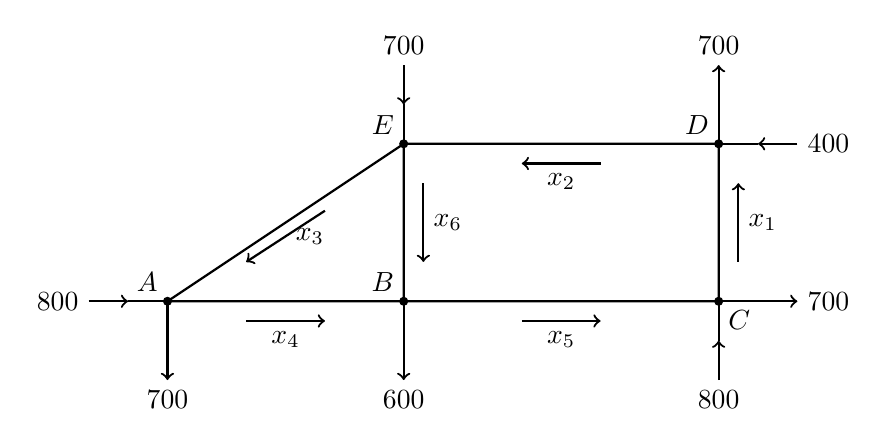
\begin{tikzpicture}
            \draw[thick, ->] (0,0) node[anchor=east]{800} -- (0.5,0);
            \draw[thick] (0.5,0) -- (1,0);
            \draw[thick] (1,0) -- (8,0);
            \draw[thick,->] (1,0) -- (1,-1) node[anchor=north]{$700$};
            \draw[thick] (1,-0.5) -- (1,0);
            \draw[thick] (1,0) -- (4,0) -- (8,0) -- (8,2) -- (4,2) -- (1,0) -- (4,0) --
            (4,2);
            \draw[fill=black] (1,0) node[anchor=south east]{$A$} circle(0.05cm);
            \draw[fill=black] (4,0) node[anchor=south east]{$B$} circle(0.05cm);
            \draw[fill=black] (8,0) node[anchor=north west]{$C$} circle(0.05cm);
            \draw[fill=black] (8,2) node[anchor=south east]{$D$} circle(0.05cm);
            \draw[fill=black] (4,2) node[anchor=south east]{$E$} circle(0.05cm);
            \draw[thick, ->] (4,0) -- (4,-1) node[anchor=north]{600};
            \draw[thick,->] (8,-1) node[anchor=north]{800} -- (8,-0.5);
            \draw[thick] (8,-0.5) -- (8,0);
            \draw[thick,->] (8,0) -- (9,0) node[anchor=west]{700};
            \draw[thick,->] (9,2)  node[anchor=west]{400} -- (8.5,2);
            \draw[thick] (8.5,2) -- (8,2);
            \draw[thick,->] (8,2) -- (8,3)  node[anchor=south]{700};
            \draw[thick,->] (4,3)  node[anchor=south]{700} -- (4,2.5);
            \draw[thick] (4,2.5) -- (4,2);
            \draw[thick, ->] (2,-0.25) -- (3,-0.25) node[midway, below]{$x_4$};
            \draw[thick, ->] (5.5,-0.25) -- (6.5,-0.25) node[midway, below]{$x_5$};
            \draw[thick, ->] (8.25,0.5) -- (8.25,1.5) node[midway, right]{$x_1$};
            \draw[thick, ->] (6.5,1.75) -- (5.5,1.75) node[midway, below]{$x_2$};
            \draw[thick, ->] (4.25,1.5) -- (4.25,0.5) node[midway, right]{$x_6$};
            \draw[thick, ->] (3,1.15) -- (2,0.5) node[midway, right]{$x_3$};
        \end{tikzpicture}
    \end{center}
    \begin{enumerate}
        \item[(a)] Write a system of 5 equations with 6 unknowns.  Each equation should
            correspond to a node in the traffic graph and each unknown corresponds to the
            flow of traffic along a road.
        \item[(b)] Solve the system of equations using software.
        \item[(c)] You should notice that the system of equations has infinitely many
            solutions.  Write the parametric form of the solution.
        \item[(d)] What does each vector in the parametric form tell us about the traffic
            graph?
    \end{enumerate}
\end{problem}



\begin{definition}[Row Space]
        Let $A$ be an $m \times n$ matrix. The subspace of $\mathbb{R}^n$ spanned by the
        $m$ rows of $A$ is called the {\bf row space} of $A$
\end{definition}

\begin{problem}
    What is the row space of the traffic problem matrix from Problem \ref{prob:traffic}
    and what does it have to do with the context of traffic flow?
\end{problem}

\begin{definition}[Row Rank of a Matrix]
    The dimension of the row space is called the (row) {\bf rank} of the matrix $A$
\end{definition}

\begin{problem}
    What is the row rank of the traffic problem matrix from Problem \ref{prob:traffic}?
\end{problem}

\begin{definition}[Column Space]
        Let $A$ be an $m \times n$ matrix. The subspace of $\mathbb{R}^m$ spanned by the
        $n$ column vectors is called the {\bf column space} of $A$.
\end{definition}
\begin{problem}
    What is the column space of the traffic problem depicted in Problem \ref{prob:traffic}
    and what does it have to do with the context of traffic flow?
\end{problem}

\begin{definition}[Column Rank of a Matrix]
    The dimension of the column space a matrix $A$ is called the (column) {\bf rank} of $A$.
\end{definition}
\begin{problem}
    What is the column rank of the traffic problem matrix from Problem \ref{prob:traffic}?
\end{problem}

\begin{definition}[Null Space (Kernel)]
        Let $A$ be an $m \times n$ matrix.  The {\bf null space} os a matrix $A$ is the
        solution space of the homogeneous system $A \bx = \bo$ 
        \[ Null(A) = \{ \bx \, : \,
        A\bx = \bo \} \]
        The null space of a matrix $A$ is often denoted $Null(A)$ of $\mathcal{N}(A)$.  We
        will use both interchangeably throughout the remainder of these notes.
\end{definition}
\begin{problem}
    What is the null space of the traffic problem depicted in Problem \ref{prob:traffic}
    and what does it have to do with the context of traffic flow?  Pay particular
    attention here to the situation where only the roads indicated in the null space are
    turned on.  What do you see in the traffic pattern?  
\end{problem}

\begin{definition}[Nullity of a Matrix]
    The dimension of the null space of a matrix $A$ is called the {\bf nullity} of $A$.
\end{definition}
\begin{problem}
    What is the nullity of the traffic problem matrix from Problem \ref{prob:traffic}?
\end{problem}

\begin{thm}
    In the previous definitions we explicitly stated that each of the spaces are indeed
    subspaces.  More specifically, if $A$ is an $m \times n$ matrix then
    \begin{enumerate}
        \item[(a)] the span of the rows of $A$ is a subspace of $\mathbb{R}^n$
        \item[(b)] the span of the columns of $A$ is a subspace of $\mathbb{R}^m$
        \item[(c)] the set $\mathcal{N}(A) = \{\bx \, : \, A\bx = \bo\}$ is a subspace of
            $\mathbb{R}^n$.
    \end{enumerate}
\end{thm}
\begin{proof}
    (you should prove all three of these statements)
\end{proof}
\solution{
    \begin{proof}
        \begin{enumerate}
            \item[(a)] The rows of the matrix $A$ contain $n$ entries so they are elements of
                $\mathbb{R}^n$.  The span of a collection of vectors is always a subspace by
                Theorem \ref{thm:span_subspace} so the span of the rows of $A$ is a
                subspace of $\mathbb{R}^n$.
            \item[(b)] The columns of the matrix $A$ contain $m$ entries so they are elements of
                $\mathbb{R}^m$.  The span of a collection of vectors is always a subspace by
                Theorem \ref{thm:span_subspace} so the span of the rows of $A$ is a
                subspace of $\mathbb{R}^m$.
            \item[(c)] First observe that any $\bx \in \mathcal{N}(A)$ are vectors in
                $\mathbb{R}^n$ since the matrix multiplication $A \bx = \bo$ must make
                sense.  Let $\bx_1, \bx_2 \in \mathcal{N}(A)$ and let $c_1, c_2 \in
                \mathbb{R}$.  Observe that if we multiply the linear combination $c_1
                \bx_1 + c_2 \bx_2$ by the matrix $A$ we get
                \[ A \left( c_1 \bx_1 + c_2 \bx_2 \right) = c_1 A \bx_1 + c_2 A \bx_2 =
                c_1 \bo + c_2 \bo = \bo \]
                so we conclude that the linear combination is in the null space of $A$.
                Hence, by Theorem \ref{thm:prove_subspace} we have shown that the null
                space is indeed a subspace of $\mathbb{R}^n$.
        \end{enumerate}
    \end{proof}
}


\begin{problem}
    Find a basis for the null, column, and row spaces for the matrix below.  The row
    reduced form of the matrix is given for convenience.
    \[ A = \begin{pmatrix} 5 & -2 & 3 \\ -1 & 0 & -1 \\ 0 & -2 & -2 \\ -5 & 7 & 2
    \end{pmatrix} \to \cdots \to \begin{pmatrix}
            1 & 0 & 1 \\ 0 & 1 & 1 \\ 0 & 0 & 0 \\ 0 & 0 & 0 
        \end{pmatrix} \]
\end{problem}
\solution{
    \begin{flalign*}
        Nul(A) &= span\left\{ \begin{pmatrix} -1\\-1\\1\end{pmatrix} \right\} \\
        Col(A) &= span\left\{ \begin{pmatrix} 5\\-1\\0\\-5\end{pmatrix} ,
        \begin{pmatrix} -2\\0\\-2\\7\end{pmatrix} \right\} \\
        Row(A) &= span\left\{ \begin{pmatrix} 1\\0\\1 \end{pmatrix} ,
        \begin{pmatrix} 0\\1\\1 \end{pmatrix} \right\} 
    \end{flalign*}
}


\begin{problem}
    True or False:
    \begin{itemize}
        \item[(a)] If $A$ is a $2 \times 3$ matrix then the zero vector $\bo = \begin{pmatrix} 0\\0
            \end{pmatrix}$ is in the column space of $A$.
        \item[(b)] If $A$ is a $2 \times 3$ matrix then the zero vector $\bo = \begin{pmatrix} 0\\0
            \end{pmatrix}$ is in the row space of $A$.
        \item[(c)] If $A$ is a $2 \times 3$ matrix then the zero vector $\bo = \begin{pmatrix} 0\\0
            \end{pmatrix}$ is in the null space of $A$.
    \end{itemize}
\end{problem}
\solution{
    \begin{enumerate}
        \item[(a)] True
        \item[(b)] False
        \item[(c)] False
    \end{enumerate}
}

\begin{example}
    Find the row space, column space, and null space of the matrix 
    \[ A = \begin{pmatrix} -3 & 6 & -1 & 1 & -7 \\ 1 & -2 & 2 & 3 & -1 \\ 2 & -4 & 5 & 8 &
        -4 \end{pmatrix}. \]
    Also find the rank and the nullity.
    {\bf Solution:} First we observe that $A$ row reduces to 
    \[ A \to \cdots \to \begin{pmatrix} 1 & -2 & 0 & -1 & 3 \\ 0 & 0 & 1 & 2 & -2 \\ 0 & 0
        & 0 & 0 & 0 \end{pmatrix}. \]
    \begin{description}
        \item[Column Space:] We observe that columns 1 and 3 are linearly independent so
            the column space of $A$ is 
            \[ \text{Col}(A) = \text{span}\left( \begin{pmatrix} -3 \\ 1 \\ 2
                \end{pmatrix} \, , \, \begin{pmatrix} -1 \\ 2 \\ 5 \end{pmatrix} \right)
            \]
            which is a subspace of $\mathbb{R}^3$.\\
            (Notice that we are NOT claiming that the column space is the span of the
            first and third columns from the row reduced matrix.  Why?)
        \item[Row Space:] From the row reduced form we see that columns 1 and 2 are
            linearly independent.  Since the row reduced form of $A$ is ``row equivalent''
            we see that the row space of $A$ is
            \[ \text{Row}(A) = \text{span}\left( (1,-2,0,-1,3) \, , \, (0,0,1,2,-2)
            \right) \]
            which is a subspace of $\mathbb{R}^5$.
        \item[Null Space:] For the null space we are considering the equation $A \bx =
            \bo$.  From the row reduced form of the matrix we see that the solution to the
            homogeneous system is
            \begin{flalign*}
                x_1 &= 2x_2 + x_4 - 3x_5 \\
                x_3 &= -2 x_4 + 2x_5
            \end{flalign*}
            where $x_2, x_4, x_5 \in \mathbb{R}$.  Therefore we can write the solution to
            the homogeneous system as
            \[ \begin{pmatrix} x_1 \\ x_2 \\ x_3 \\ x_4 \\ x_5 \end{pmatrix} =
                \begin{pmatrix} 2 \\ 1 \\ 0 \\ 0 \\ 0 \end{pmatrix} x_2 + \begin{pmatrix}
                    1 \\ 0 \\ -2 \\ 1 \\ 0 \end{pmatrix} x_4 + \begin{pmatrix} -3 \\ 0 \\
                2 \\ 0 \\ 1 \end{pmatrix}x_5 \]
            Thus the null space of $A$ is
            \[ \mathcal{N}(A) = \text{span}\left( \begin{pmatrix} 2 \\ 1 \\ 0 \\ 0 \\ 0
                \end{pmatrix} \, , \, \begin{pmatrix}
                    1 \\ 0 \\ -2 \\ 1 \\ 0 \end{pmatrix} \, , \, \begin{pmatrix} -3 \\ 0 \\
                2 \\ 0 \\ 1 \end{pmatrix} \right) \]
            which is a subspace of $\mathbb{R}^5$.
        \item[Rank:] The rank is the dimension of the column space.  We see that the basis
            of the column space has 2 vectors so $\text{rank}(A) = 2$.
        \item[Nullity:] The nullity is the dimension of the null space.  We see that the
            basis for the 
            null space has three vectors so $\text{nullity}(A) = 3$.  Observe that 
            \[ \text{rank}(A) + \text{nullity}(A) = 5 = \text{number of columns in $A$}. \]
    \end{description}
\end{example}




\begin{example}
    Let $A = \begin{pmatrix} 0 & 1 & 0 \\ 0 & 0 & 1 \\ 0 & 0 & 0 \end{pmatrix}$.  Find
    $\mathcal{N}(A)$ and determine the nullity of $A$.\\
    {\bf Solution: } This matrix is already row reduced so we can read the solution to the
    homogeneous system $A \bx = \bo$ as $x_2 = 0$, $x_3 = 0$ and $x_1 \in \mathbb{R}$.
    Therefore,
    \[ \mathcal{N}(A) = \text{span}\left( \begin{pmatrix}1\\0\\0\end{pmatrix} \right) \]
    Since the basis for the null space has only one vector we see that $\text{nullity}(A)
    = 1$.  One might also observe that $\text{rank}(A) = 2$ and that $\text{rank}(A) +
    \text{nullity}(A) = 3$ which is the number of columns in $A$.
\end{example}

\begin{example}
    Let $A$ be a matrix that row reduces to $A \to \cdots \to \begin{pmatrix} 0 & 1 & 0 \\
        0 & 0 & 1 \\ 0 & 0 & 0 \end{pmatrix}$.  Describe $\text{Col}(A)$ and determine the
    rank of $A$.\\
    {\bf Solution: } The column space is
    the span of columns 2 and 3 since these are the two linearly independent columns.
    Since the basis for the column space contains two vectors we see that $\text{rank}(A)
    = 2$.  
\end{example}

\begin{example}
    Consider the matrix 
    \[ A = \begin{pmatrix} 1 & 2 & 3 \\ 4 & -1 & \pi \\ -30 & 1 & 17 \\ 19 & 3 & -e^2 \\ 0
        & 0 & 2 \end{pmatrix} \]
    The row, column, and null spaces are subspaces of which vector spaces? \\
    {\bf Solution:} 
    \begin{description}
        \item[Row Space: ] The row space is a subspace of $\mathbb{R}^3$ since each row
            contains three entries.
        \item[Column Space: ] The column space is a subspace of $\mathbb{R}^5$ since each
            column contains 5 entries.
        \item[Null Space: ] The null space is a subspace of $\mathbb{R}^3$ since for $\bx
            \in \text{Null}(A)$ the equation $A\bx = \bo$ must make sense.  Since
            $A$ is a $5 \times 3$ matrix $\bx$ must be a $3 \times 1$ vector.
    \end{description}
\end{example}

\begin{problem}
    The \textit{row space} of a matrix $A$ is the set of vectors that can be created
    by taking all linear combinations of the rows of $A$.  Which of the following vectors is in
    the row space of the matrix 
    $A=\left( \begin{array}{cc} 1 & 2\\ 3 & 6 \\ \end{array} \right)$?

\begin{enumerate}
    \item[(a)] $\bx=\left( \begin{array}{cc} -2& 4\\ \end{array} \right)$
\item[(b)] $\bx=\left( \begin{array}{cc} 4& 8\\ \end{array} \right)$
\item[(c)] $\bx=\left( \begin{array}{cc} 0& 0\\ \end{array} \right)$
\item[(d)] $\bx=\left( \begin{array}{cc} 8& 4\\ \end{array} \right)$ 
\item[(e)] More than one of the above
\item[(f)] None of the above
\end{enumerate}
\end{problem}
\solution{(e)}

% \begin{problem}
%     \begin{itemize}
%             \input{ClickerQuestions/LA.00.16.080}
%     \end{itemize}
% \end{problem}
% \solution{
% 5
% }

\begin{problem}
    The \textit{column space} of a matrix $A$ is the set of vectors that can be created
    by taking all linear combinations of the columns of $A$.  Is the vector 
    $\bb=\left( \begin{array}{c} -4\\ 12\\ \end{array} \right)$
    in the column space of the matrix
    $A=\left( \begin{array}{cc} 1 & 2\\ 3 & 6 \\ \end{array} \right)$?
\begin{enumerate}
    \item[(a)] Yes, since we can find a vector $\bx$ so that $A\bx=\bb$.
    \item[(b)] Yes, since $-2\left( \begin{array}{c} 1\\ 3\\ \end{array} \right) 
-1 \left( \begin{array}{c} 2\\ 6\\ \end{array} \right) =
\left( \begin{array}{c} -4\\ 12\\ \end{array} \right)$.
\item[(c)] No, because there is no vector $\bx$ so that $A\bx=\bb$.
\item[(d)] No, because we can't find $c_1$ and $c_2$ such that
$c_1\left( \begin{array}{c} 1\\ 3\\ \end{array} \right) 
+ c_2 \left( \begin{array}{c} 2\\ 6\\ \end{array} \right) =
\left( \begin{array}{c} -4\\ 12\\ \end{array} \right)$. 
\item[(e)] More than one of the above
\item[(f)] None of the above
\end{enumerate}
\end{problem}
\solution{
No (c and d)
}
% 
% \begin{problem}
%     \begin{itemize}
%             \input{ClickerQuestions/LA.00.16.020}
%     \end{itemize}
% \end{problem}


\begin{problem}
    \textbf{True or False:} The row space of a matrix $A$ is the same as the column space of $A^T$.
\end{problem}
\solution{True}

% \begin{problem}
%     \begin{itemize}
%             \input{ClickerQuestions/LA.00.16.090}
%     \end{itemize}
% \end{problem}
% \solution{
% True
% }


\begin{problem}
    The row space of the matrix
$A=\left( \begin{array}{cc} 1 & 2\\ 3 & 6 \\ \end{array} \right)$ consists of
\begin{enumerate}
    \item[(a)] All linear combinations of the columns of $A^T$.
\item[(b)] All multiples of the vector $\left( \begin{array}{c} 1\\ 2\\ \end{array} \right)$. 
\item[(c)] All linear combinations of the rows of $A$.
\item[(d)] All of the above
\item[(e)] None of the above
\end{enumerate}
\end{problem}
% 
% \begin{problem}
%     \begin{itemize}
%             \input{ClickerQuestions/LA.00.16.100}
%     \end{itemize}
% \end{problem}
\solution{
d
}

\begin{problem}
    The column space of the matrix 
$A=\left( \begin{array}{cc} 1 & 2\\ 3 & 6 \\ \end{array} \right)$ is
\begin{enumerate}
    \item[(a)] the set of all linear combinations of the columns of $A$.
    \item[(b)] a line in $\Re^2$.
    \item[(c)] the set of all multiples of the vector $\left( \begin{array}{c} 1\\ 3\\ \end{array} \right)$. 
    \item[(d)] All of the above
    \item[(e)] None of the above
\end{enumerate}
\end{problem}
% \begin{problem}
%     \begin{itemize}
%             \input{ClickerQuestions/LA.00.16.030}
%     \end{itemize}
% \end{problem}
\solution{
d
}





\begin{problem}
    The \textit{null space} of a matrix $A$ is the set of all vectors $x$ that are solutions of
    $Ax=0$.  Which of the following vectors is in the null space of the matrix  
    $A=\left( \begin{array}{cc} 1 & 2\\ 3 & 6 \\ \end{array} \right)$?
\begin{enumerate}
    \item[(a)] $x=\left( \begin{array}{c} -2\\ 1\\ \end{array} \right)$
    \item[(b)] $x=\left( \begin{array}{c} 0\\ 0\\ \end{array} \right)$
    \item[(c)] $x=\left( \begin{array}{c} 4\\ -2\\ \end{array} \right)$ 
    \item[(d)] All of the above
    \item[(e)] None of the above
\end{enumerate}
\end{problem}
% \begin{problem}
%     \begin{itemize}
%             \input{ClickerQuestions/LA.00.16.060}
%     \end{itemize}
% \end{problem}
\solution{
d
}


\begin{problem}
    Let $A =
    \left( \begin{array}{cccc}
            1 & 0 & 2 & 1\\
            0 & 1 & 3 & 1\\
        2 & -1 & 1 & 1\end{array} \right).$
    Which of the following vectors are in the nullspace of $A$?

\begin{enumerate}
    \item[(a)]  
        $\left( \begin{array}{c} -2 \\ 0 \\ -1 \end{array} \right)$
    \item[(b)]  
        $\left( \begin{array}{c} 3 \\ 3 \\ 3 \end{array} \right)$
    \item[(c)]  
        $\left( \begin{array}{c} 2 \\ 3 \\ -1 \\ 0 \end{array} \right)$
    \item[(d)]  
        $\left( \begin{array}{c} 3 \\ -1 \\ 3 \\ 2 \end{array} \right)$
\end{enumerate}
\end{problem}
% \begin{problem}
%     \begin{itemize}
%             \input{ClickerQuestions/LA.00.16.150}
%     \end{itemize}
% \end{problem}
\solution{
c
}



\begin{thm}[Rank-Nullity Theorem]
    Let $A$ be an $m \times n$ matrix.  The sum of the rank and the nullity of $A$ is the
    number of columns of $A$.
    \[ \text{dimension}(\text{Null}(A)) + \text{dimension}(\text{Col}(A)) = n \]
\end{thm}

\newpage
\section{The Invertible Matrix Theorem}
\begin{problem}
    Let $A$ be an $n \times n$ square matrix and assume that $A$ is invertible.  Mark each
    of the following statements about the matrix $A$ as either true or false. If a
    statement is true then prove it.  If a statement is false then provide a
    counterexample.
    \begin{enumerate}
        \item[(a)] $\det(A) \ne 0$ \vfill
        \item[(b)] $A$ can be row reduced to the $n \times n$ identity matrix \vfill
        \item[(c)] $A$ has $n$ pivot positions \vfill
        \item[(d)] The equation $A \bx = \bo$ has only the trivial solution \vfill
        \item[(e)] The columns of $A$ form a linearly independent set \vfill
        \item[(f)] The equation $A \bx = \bb$ has at least one solution for each $\bb \in
            \mathbb{R}^n$ \vfill
        \item[(g)] The columns of $A$ span $\mathbb{R}^n$ \vfill
        \item[(h)] There is an $n \times n$ matrix $C$ such that $CA = I$ \vfill
        \item[(i)] There is an $n \times n$ matrix $D$ such that $AD = I$ \vfill
        \item[(j)] $A^T$ is invertible \vfill
        \item[(k)] The columns of $A$ form a basis for $\mathbb{R}^n$ \vfill
        \item[(l)] $\text{Col}(A) = \mathbb{R}^n$ \vfill
        \item[(m)] $\text{dim}(\text{Col}(A)) = n$ \vfill
        \item[(n)] $\text{rank}(A) = n$ \vfill
        \item[(o)] $\text{Null}(A) = \{ \bo \}$ \vfill
        \item[(p)] $\text{dim}(\text{Null}(A)) = 0$ \vfill
    \end{enumerate}
\end{problem}

\begin{problem}
    If we assume that $A$ is \underline{not} invertible in the previous problem then which
    statements would be true and which would be false? Be able to defend your answers.
\end{problem}

\newpage


As you undoubtedly found in the previous problem, all of the statements are true under the
assumption that $A$ was invertible.  We can
actually morph this into a more powerful theorem about matrices.  
\begin{thm}[Invertible Matrix Theorem]
    Let $A$ be an $n \times n$ square matrix.  Then the following statements are
    equivalent.  That is, for a given matrix $A$, \\
    \underline{the following statements are either {\bf all true or
    all false}.}
    \begin{enumerate}
        \item[(a)] $A$ is an invertible matrix
        \item[(b)] $A$ can be row reduced to the $n \times n$ identity matrix
        \item[(c)] $A$ has $n$ pivot positions
        \item[(d)] The equation $A \bx = \bo$ has only the trivial solution
        \item[(e)] The columns of $A$ form a linearly independent set
        \item[(f)] The equation $A \bx = \bb$ has at least one solution for each $\bb \in
            \mathbb{R}^n$
        \item[(g)] The columns of $A$ span $\mathbb{R}^n$
        \item[(h)] There is an $n \times n$ matrix $C$ such that $CA = I$
        \item[(i)] There is an $n \times n$ matrix $D$ such that $AD = I$
        \item[(j)] $A^T$ is invertible
        \item[(k)] The columns of $A$ form a basis for $\mathbb{R}^n$
        \item[(l)] $\text{Col}(A) = \mathbb{R}^n$
        \item[(m)] $\text{dim}(\text{Col}(A)) = n$
        \item[(n)] $\text{rank}(A) = n$
        \item[(o)] $\text{Null}(A) = \{ \bo \}$
        \item[(p)] $\text{dim}(\text{Null}(A)) = 0$
        \item[(q)] $\det(A) \ne 0$
    \end{enumerate}
\end{thm}

\begin{problem}
    Consider the following true or false questions.
    \begin{enumerate}
        \item[(a)] The number of free variables in the solution to $A \bx = \bo$ is equal
            to the dimension of the null space of $A$. \solution{True}
        \item[(b)] If $A$ is a $3 \times 4$ matrix then the row vectors belong to
            $\mathbb{R}^3$. \solution{False, they belong to $\mathbb{R}^4$}
        \item[(c)] If $A$ is an $n \times n$ matrix and $A \bx = \bo$ has only the trivial
            solution, then the dimension of the null space of $A$ is 0. \solution{True}
        \item[(d)] If $S$ is a set of three vectors, each of these is in $\mathbb{R}^2$,
            then $S$ spans $\mathbb{R}^2$. \solution{False, they could form a
                1-dimensional subspaces of $\mathbb{R}^2$}
        \item[(e)] If $A$ is an $n\times n$ matrix and the dimension of the null space is
            0 then $A$ is invertible. \solution{True}
    \end{enumerate}
\end{problem}

\begin{problem}
    If $A$ is an $n \times n$ matrix and $A \bx = \bb$ has a solution for all $\bb \in
    \mathbb{R}^n$ then which of the following are true?
    \begin{itemize}
        \item $A$ is invertible
        \item The columns of $A$ are linearly independent
        \item $A \bx = \bo$ has only the trial solution
        \item The columns of $A$ span $\mathbb{R}^n$
    \end{itemize}
\end{problem}
\solution{
All of them are true.
}


\begin{problem}
    Consider the matrix $A = \begin{pmatrix} 1 & -1 & 0 \\ -1 & 2 & 2 \\ 0 & 2 & 4
    \end{pmatrix}$.  It can be shown that $\det(A) = 0$.  Based on this fact find all of
    the following statements that must be true about $A$.
    \begin{itemize}
        \item[(a)] The matrix $A$ is invertible.
        \item[(b)] The columns of $A$ are linearly dependent.
        \item[(c)] The columns of $A$ form a basis for $\mathbb{R}^3$.
        \item[(d)] The rank of $A$ is less than $3$
        \item[(e)] $A \bx = \bo$ ha a non-trivial solution.
    \end{itemize}
\end{problem}
\solution{
(b), (d), and (e) are true
}

\newpage\section{Additional Exercises}

\begin{problem}
    For each True/False question be able to give a proof or counterexample to support your
    answer.
    \begin{enumerate}
        \item[(a)] True or False: If an $n \times n$ matrix has a determinant of zero then
            its columns are linearly independent. \solution{False}
        \item[(b)] True or False: If $A$ is a $2 \times 3$ matrix then the zero vector $\bo =
            \begin{pmatrix}0\\0\end{pmatrix}$ is in the column space of $A$.
            \solution{True}
        \item[(c)] True or False: If $A$ is a $2 \times 3$ matrix then the zero vector $\bo =
            \begin{pmatrix}0\\0\end{pmatrix}$ is in the row space of $A$.
            \solution{False but the zero vector $\bo = (0,0,0)^T$ is in the row space}
        \item[(d)] True or False: A set of 5 vectors in $\mathbb{R}^4$ spans all of
            $\mathbb{R}^3$. \solution{false}
        \item[(e)] True or False: If $A$ is an $n \times n$ matrix and $A$ is invertible
            then the sum of the dimensions of the row and null spaces of $A$ is equal to
            $n$. \solution{True}
        \item[(f)] True or False: The span of a set of vectors is a subspace of some vector
            space.  \solution{True}
        \item[(g)] True or False: the matrix $A = \begin{pmatrix} 1 & 0 & 2 \\ 0 & 3 & -2
                \\ 0 & 0 & 4\end{pmatrix}$ is invertible. \solution{True, the determinant
            is $\det(A) = 1 \cdot 3 \cdot 4 \ne 0$} 
        \item[(h)] True or False: If $A^{-1}$ does not exist then the null space contains
            only the zero vector. \solution{False}
        \item[(i)] If $A$ is an $n \times n$ square matrix and $A^T$ is invertible then
            $A\bx = \bo$ has infinitely many solutions. \solution{False.  IF $A^T$ is
                invertible then $A$ is invertible so $A\bx = \bo$ has only the trivial
            solution.}
    \end{enumerate}
\end{problem}

\begin{problem}
    Which set of vectors is linearly independent?
    \begin{enumerate}
        \item[(a)] $(2,3)$, $(8,12)$
        \item[(b)] $(1,2,3)$, $(4,5,6)$, $(7,8,9)$
        \item[(c)] $(-3,1,0)$, $(4,5,2)$, $(1,6,2)$
        \item[(d)] None of these sets are linearly independent.
        \item[(e)] Exactly two of these sets are linearly independent.
        \item[(f)] All of these sets are linearly independent.
    \end{enumerate}
\end{problem}
\solution{
None of these are linearly independent.  You can tell by row reducing each of them.
\begin{flalign*}
    &1: \quad \begin{pmatrix} 2 & 8 \\ 3 & 12 \end{pmatrix} \to \begin{pmatrix} 1 & 4 \\ 0
        & 0 \end{pmatrix} \\
    &2: \quad \begin{pmatrix} 1 & 4 & 7 \\ 2 & 5 & 8 \\ 3 & 6 & 9 \end{pmatrix} \to
    \begin{pmatrix} 1 & 0 & -1 \\ 0 & 1 & 2 \\ 0 & 0 & 0 \end{pmatrix} \\
    &3: \quad \begin{pmatrix} -3 & 4 & 1 \\ 1 & 5 & 6 \\ 0 & 2 & 2 \end{pmatrix} \to
    \begin{pmatrix} 1 & 0 & 1 \\ 0 & 1 & 1 \\ 0 & 0 & 0 \end{pmatrix}
\end{flalign*}
}

% \begin{problem}
%     \begin{itemize}
%             \input{ClickerQuestions/LA.00.06.010} 
%     \end{itemize}
% \end{problem}
% \solution{
% }


\begin{problem}
    Let $\bv_1 = \begin{pmatrix} 1 \\ 1 \\ 2 \end{pmatrix}$, $\bv_2 = \begin{pmatrix} 3 \\
        0 \\ -1 \end{pmatrix}$, and $\bv_3 = \begin{pmatrix} 6 \\ 0 \\ -2 \end{pmatrix}$.
            Geometrically, what is the subspace spanned by the set $\{\bv_1, \bv_2,
            \bv_3\}$?\\
        (a) a point, \quad
        (b) a line, \quad  
        (c) a plane, \quad 
        (d) a volume, \quad   
        (e) All of $\mathbb{R}^3$.
\end{problem}
\solution{A plane}

% \begin{problem}
%     \begin{itemize}
%             \input{ClickerQuestions/LA.00.15.265}
%             Follow up: What is a basis for the subspace?
%     \end{itemize}
% \end{problem}
% \solution{3
% }


\begin{problem}
    Which of the follow sets are subspaces of $\mathbb{R}^3$?
    \begin{flalign*}
        S_1 &= \left\{ (x,y,z) \, : \, x+y+z=7 \right\} \\
        S_2 &= \left\{ (x,y,z) \, : \, x+y+z=0 \right\} \\
        S_3 &= \left\{ (x,y,z) \, : \, -3x-4y=0, \text{ and } -9x+7z = 0 \right\} \\
        S_4 &= \left\{ (7x+8y , -5x+2y, -6x-2y) \, : \, x,y \in \mathbb{R} \right\} \\
        S_5 &= \left\{ (3,y,z) \, : \, y,z\in\mathbb{R} \right\} \\
        S_6 &= \left\{ (x,y,z) \, : \, x,y,z>0 \right\} \\
    \end{flalign*}
\end{problem}
\solution{
    Hint: Pick arbitrary elements in the sets and check that scalar multiples of these
    elements as well as sums of these elements are still in the set.
}


\begin{problem}
    We say that a vector $\bv$ is in the span of a set of vectors if $\bv$ can e written
    as a linear combination of the vectors in the set.  Let
    \[ \bv_1 = \begin{pmatrix} 4 \\ 4 \\ -2 \end{pmatrix} \quad \bv_2 = \begin{pmatrix} -4
            \\ -6 \\ 4 \end{pmatrix} \quad \text{and} \quad \begin{pmatrix} 4 \\ 12 \\ h
            \end{pmatrix}. \]
    For what value of $h$ is $\bv_3$ in the plane spanned by $\bv_1$ and $\bv_2$?
\end{problem}
\solution{
    Hint: If $\bv_3$ is in the plane spanned by $\bv_1$ and $\bv_2$ then $\bv_3$ can be
    written as a linear combination of $\bv_1$ and $\bv_2$. 
}

\begin{problem}
    Find a linearly independent spanning set for the subspace of $\mathbb{R}^3$ defined by
    the equation $8x_1 + 7x_2 - 6x_3 = 0$.  You should also notice that this is the
    equation of a plane.  Give a vector that is perpendicular to the plane.
\end{problem}
\solution{
    Hint: Think of the equation $8x_1 + 7x_2 - 6x_3 = 0$ as the solution to a homogeneous
    system of equations with 1 equation and 3 unknowns.  Clearly there are two free
    variables ($x_2$ and $x_3$) so you can choose them arbitrarily giving two independent
    vectors that span the plane.  
}

\begin{problem}
    Find a basis of the subspace of $\mathbb{R}^5$ spanned by the vectors
    \[ \begin{pmatrix} 2\\1\\1\\0\\3\end{pmatrix},
        \begin{pmatrix}7\\0\\7\\-6\\14\end{pmatrix},
        \begin{pmatrix}-3\\2\\-5\\7\\-8\end{pmatrix},
        \begin{pmatrix}2\\1\\2\\0\\3\end{pmatrix},
        \begin{pmatrix}4\\2\\4\\0\\6\end{pmatrix} \]
\end{problem}
\solution{
    Hint: Which vectors and linearly independent of the others?
}

\begin{problem}
    Consider the matrix $A = \begin{pmatrix} 1 & -1 & 0 \\ -1 & 2 & 2 \\ 0 & 2 & 4
    \end{pmatrix}$.  It can be shown that $\det(A) = 0$.  Based on this fact determine
    whether the following statements are true or false.
    \begin{enumerate}
            \item[(a)] True or False: The matrix $A$ is invertible.
            \solution{
                False
            }
            \item[(b)] True or False: The columns of $A$ are linearly dependent.
            \solution{
                True
            }
            \item[(c)] True or False: The columns of $A$ form a basis for $\mathbb{R}^3$.
            \solution{
                False
            }
            \item[(d)] True or False: The rank of $A$ is less than 3.
            \solution{
                True
            }
            \item[(e)] True or False: The equation $A \bx = \bo$ has a non-trivial solution.
            \solution{
                True
            }
    \end{enumerate}
\end{problem}


\begin{problem}
    Let $A$ be an $n \times n$ matrix and assume that $A \bx = \bb$ has a
    unique solution for all
    $\bb \in \mathbb{R}^n$.
    \begin{enumerate}
        \item[(a)] True or False: $A$ is invertible. 
        \solution{
            True
        }
        \item[(b)] True or False: The columns of $A$ are linearly dependent. 
        \solution{
            False
        }
        \item[(c)] True or False: $A \bx = \bo$ has only the trivial solution.
        \solution{
            True
        }
        \item[(d)] True or False: The columns of $A$ span $\mathbb{R}^n$
        \solution{
            True
        }
    \end{enumerate}
\end{problem}
\begin{problem}
 Mark True or False.  Do not assume that the matrix $A$ is square unless stated so in the
 question. 
    \begin{enumerate}
        \item[(a)] True or False: The number of free variables in the solution to $A \bx =
        \bo$ is equal to the dimension of the column space of $A$.
        \solution{
            False
        }
        \item[(b)] True or False: If $A$ is a $3 \times 4$ matrix then the row vectors belong to
        $\mathbb{R}^3$.
        \solution{
            False.  They belong to $\mathbb{R}^4$.
        }
        \item[(c)] True or False: If $A$ is $n \times n$ and $A \bx = \bo$ has only the
        trivial solution, then the dimension of the null space of $A$ is greater than 0.
        \solution{
            False
        }
        \item[(d)] True or False: If $S$ is a set of three vectors, each of which is in
        $\mathbb{R}^2$, then $S$ spans $\mathbb{R}^2$.
        \solution{
            False.  Two of the three could just be scalar multiples of the other one hence
            letting $S$ span a 1-D subspace of $\mathbb{R}^2$.
        }
        \item[(e)] True or False: If $A$ is an $n \times n$ matrix and the dimension of the
        null space is 0 then $A$ is invertible.
        \solution{
            True
        }
    \end{enumerate}

\end{problem}

\begin{problem}
    Find the null space, row space, and column space for the matrix
    \[ A = \begin{pmatrix} 4 & -1 & 3 \\ 12 & -6 & 9 \\ -4 & 2 & -3 \end{pmatrix} \]
\end{problem}


\begin{problem}
    Find a basis for each of the following vector spaces.
    \begin{enumerate}
        \item[(a)] the set of $2 \times 2$ diagonal matrices
        \item[(b)] the set of upper triangular $3 \times 3$ matrices
        \item[(c)] the set of all quadratic polynomials with no linear term
        \item[(d)] the set of all solutions to the differential equation $y' = -2y$
    \end{enumerate}
\end{problem}



\begin{problem}
    Let $\mathcal{V}$ be the set of all ordered triples $(x,y,z)$ such that $x+y+z=3$.
    Show that $\mathcal{V}$ is not a subspace of $\mathbb{R}^3$.
\end{problem}
\solution{
    $\bo \not\in \mathcal{V}$
}

\begin{problem}
    Show that every subspace $\mathcal{W}$ of a vector space $\mathcal{V}$ contains the
    zero vector.
\end{problem}
\solution{
Subspaces are closed under linear combinations so taking the zero combination puts you
back in the subspace.  Hence $\bo \in \mathcal{W}$ for all $\mathcal{W}$.
}

\begin{problem}
    Assume that the set $\{ \bv_1, \bv_2, \bv_3 \}$ is linearly independent.  Show that
    the set $\{ \bu_1, \bu_2, \bu_3\}$ is linearly independent given that
    \[ \bu_1 = \bv_2 + \bv_3, \quad \bu_2 = \bv_1 + \bv_3, \quad \bu_3 = \bv_1 + \bv_2. \]
\end{problem}
\solution{
Consider the linear combination 
\[ \bo = c_1 \bu_1 + c_2 \bu_2 + c_3 \bu_3 = c_1 (\bv_2 + \bv_3) + c_2 (\bv_1 + \bv_3) +
c_3(\bv_1 + \bv_2) = (c_2 + c_3) \bv_1 + (c_1 + c_3)\bv_2 + (c_1 + c_2)\bv_3 \]
and hence $c_1 = c_2 = c_3 = 0$.
}

\begin{problem}
    Suppose that $S$ is a set of $n$ vectors that span the $n$-dimensional vector space
    $\mathcal{V}$.  Prove that $S$ is a basis for $\mathcal{V}$.
\end{problem}
\solution{
    If $\mathcal{V}$ is $n$-dimensional then any set of $n$ vectors that spans
    $\mathcal{V}$ must also be linearly independent.  Hence, $S$ is a basis for
    $\mathcal{V}$.
}

\begin{problem}
    Explain why the $n \times n$ matrix $A$ is invertible if and only if its rank is $n$.
\end{problem}
\solution{
    If $\text{rank}(A) = n$ then $A$ has $n$ linearly independent columns and hence $A$ is
    invertible.  If $A$ is invertible then $A$ must have $n$ linearly independent columns
    meaning that the rank must be $n$.
}

\begin{problem}
    Let $\mathcal{F}$ be the space of all real-valued functions on $\mathbb{R}$.  Determine
    if the set of all functions $f$ such that $f(-x) = -f(x)$ for all $x$ is a subspace of
    $\mathcal{F}$.
\end{problem}
\solution{
    Let $f,g$ be odd functions and let $c_1,c_2 \in \mathbb{R}$.  Define $h(x) = c_1 f(x)
    + c_2 g(x)$ and consider that $h(-x) = c_1 f(-x) = c_2 g(-x) = -c_1 f(x) - c_2 g(x) =
    -h(x)$ so the set of all odd functions is a subspace of $\mathcal{F}$.
}

\begin{problem}
    Let $M_{3 \times 3}$ be the set of all $3 \times 3$ matrices.  Determine if the
    following subsets of $M_{3 \times 3}$ are subspaces
    \begin{enumerate}
        \item[(a)] The set of all diagonal $3\times 3$ matrices.
            \solution{Yes }
        \item[(b)] The set of all symmetric $3 \times 3$ matrices.
            \solution{Yes }
        \item[(c)] The set of all singular (non-invertible) $3 \times 3$ matrices
            \solution{No. For Example if we define $A$ and $B$ as
                \[ A = \begin{pmatrix} 1 & 0 & 0 \\ 0 & 0 & 0 \\ 0 & 0 & 0 \end{pmatrix}
                    \quad \text{and} \begin{pmatrix} 0 & 0 & 0 \\ 0 & 1 & 0 \\ 0 & 0 & 1
                \end{pmatrix} \]
                then $A$ and $B$ are singular but $A+B$ is not.
            }
    \end{enumerate}
\end{problem}


\begin{problem}
        Let $M_{3 \times 3}$ be the set of all real $3 \times 3$ matrices.
        Prove that the set $S$ is a subspace of $M_{3
        \times 3}$. Clearly show all of your work.
        \[ S = \left\{ \begin{pmatrix} a & 0 & 0 \\ 0 & b & 0 \\ 0 & 0 & c \end{pmatrix}
        \, : \, a,b,c \in \mathbb{R} \right\} \]
\end{problem}
\solution{
    Let $A$ and $B$ be diagonal $3 \times 3$ matrices and let $c_1, c_2 \in
    \mathbb{R}$.  The linear combination $c_1 A + c_2 B$ is also clearly a
    diagonal matrix so $S$ is a subspace of $M_{3 \times 3}$.
}

\begin{problem}
        Let $\mathcal{V}$ be the vector space of all real $2 \times 2$
        matrices and let $S$ be the subspace of all $2 \times 2$ upper triangular matrices:
    \[ S = \left\{ \begin{pmatrix} a & b \\ 0 & c \end{pmatrix} \, : \, a,b,c \in
            \mathbb{R} \right\} \]
            \begin{enumerate}
                \item[(a)] Find a basis of $S$
                \solution{
                \[ \mathcal{B} = \left\{ \begin{pmatrix} 1 & 0 \\ 0 & 0 \end{pmatrix} ,
                    \begin{pmatrix} 0 & 1 \\ 0 & 0 \end{pmatrix} ,\begin{pmatrix} 0 & 0 \\
                    0 & 1 \end{pmatrix} \right\} \]
                }
        \item[(b)] Based on your answer to part (a), what is the dimension of the
            subspace $S$?
            \solution{
                \[ dim(S) = 3 \]
            }
        \item[(c)] Explain why your basis is a basis.
            \solution{
                This is a linearly independent spanning set
            }
        \end{enumerate}

\end{problem}


\begin{problem}
    Which of the following describes the span of the set $\mathcal{V}$?
    \[ \mathcal{V} = \left\{ \begin{pmatrix} 1 \\ 2\\ 0 \end{pmatrix} \, , \, \begin{pmatrix}
        0 \\ 1\\ 2\end{pmatrix} \right\} \]
    Explain your reasoning.
\end{problem}

\begin{problem}
    Consider the set $\mathcal{V} = \left\{ \begin{pmatrix} 1 \\ 2 \\ 0\end{pmatrix} \, , \, \begin{pmatrix}
        0 \\ 1 \\ 2\end{pmatrix} \right\}$.
    \begin{enumerate}
        \item[(a)] Which of the following best describes the span of the set
            $\mathcal{V}$?
            \begin{itemize}
                \item[(i)] A point
                \item[(ii)] two points
                \item[(iii)] A line
                \item[(iv)] two lines
                \item[(v)] A plane
                \item[(vi)] A planes
                \item[(vii)] A 3 dimensional space
            \end{itemize}
        \item[(b)] Explain your reasoning from part (a).
        \item[(c)] Which of the following are in the span of $\mathcal{V}$?
            \begin{itemize}
                \item[(i)] $\begin{pmatrix}1 \\ 2 \\ 0\end{pmatrix}$
                \item[(ii)] $\begin{pmatrix} 1 \\ 2 \end{pmatrix}$
                \item[(iii)] $\begin{pmatrix} 0 \\ -2 \\ -4\end{pmatrix}$
                \item[(iv)] $\begin{pmatrix} 1 \\ 0 \\ 0\end{pmatrix}$
                \item[(v)] $3.1\begin{pmatrix} 1 \\ 2 \\ 0\end{pmatrix} - \frac{4}{5}
                    \begin{pmatrix} 0 \\ 1 \\ 2 \end{pmatrix}$
                \item[(vi)] any vector in $\mathbb{R}^3$.
            \end{itemize}
        \item[(d)] Explain in general how you can deterine if a given vector is in the
            span of some other set of vectors.
    \end{enumerate}
\end{problem}

\begin{problem}
    Suppose that $\bv_1$ and $\bv_2$ are in $\mathbb{R}^n$, $c_1$ and $c_2$ are real
    numbers, and the only solution to the vector equation $c_1 \bv_1 + c_2 \bv_2 =
    \bo$ is the trivial solutions $c_1 = c_2 = 0$.
    \begin{enumerate}
        \item[(a)] The set $\{\bv_1,\bv_2\}$ is (circle one): linearly indepenednet /
            linearly dependent.
        \item[(b)] Can $\bv_1$ be a scalar multiple of $\bv_2$?  Explain.
        \item[(c)] What is the dimension of the span of $\{\bv_1,\bv_2\}$?
    \end{enumerate}
\end{problem}

\begin{problem}
    Consider the set of vectors 
    \[ \mathcal{W} = \left\{ \begin{pmatrix}1 \\ -2 \\ 3\end{pmatrix},
        \begin{pmatrix}4\\-1\\0\end{pmatrix},
        \begin{pmatrix}3\\1\\-3\end{pmatrix},\begin{pmatrix}6\\-5\\7\end{pmatrix}
    \right\}. \]
    To detetermine whether the set is linearly independent or dependent, a student did
    the following correct row reduction:
    \[ \left(\begin{array}{cccc|c} 1&4&3&6&0\\-2&-1&1&-5&0\\3&0&-3&7&0\end{array} \right)
        \to \cdots \to \left( \begin{array}{cccc|c} 1&0&-1&0&0 \\ 0&1&1&0&0 \\
        0&0&0&1&0\end{array} \right) \]
    \begin{enumerate}
        \item[(a)] Is the set of vectors $\mathcal{W}$ linearly independent or linearly
            dependent?
        \item[(b)] Explain what it is about the row reduction matrix that tells you
            whether or not the set $\mathcal{W}$ is linearly independent or dependent.
    \end{enumerate}
\end{problem}



\begin{problem}
    The result of $\begin{pmatrix} 1&0&3\\2&1&0\end{pmatrix}
    \begin{pmatrix}-1\\2\\0\end{pmatrix}$ is (circle all that apply)
    \begin{itemize}
        \item a vector in $\mathbb{R}^2$
        \item a vector in $\mathbb{R}^3$
        \item a matrix with 2 rows and 3 columns
        \item a linear combination of vectors in $\mathbb{R}^2$
        \item a linear combination of vectors in $\mathbb{R}^3$
    \end{itemize}
\end{problem}


\begin{problem}
    The three equation below correspond to three planes in $\mathbb{R}^3$.
    \begin{flalign*}
        x+y-z&=1 \\
        x-y+z&=1 \\
        3x+y-z &= 3
    \end{flalign*}
    \begin{enumerate}
        \item[(a)] Determine if $(1,1,1)$ is a solution to the system of linear equations
            and explain how you know.
        \item[(b)] The following is the correct row reduction of the augmented matrix
            corresponding to the given system of equations:
            \[ \left( \begin{array}{ccc|c} 1&1&-1&1 \\ 1&-1&1&1 \\ 3&1&-1&3 \end{array}
                \right) \to \cdots \to \left( \begin{array}{ccc|c} 1&0&0&1 \\ 0&1&01&0 \\
                0&0&0&0 \end{array} \right). \]
            Describe all solutions to this system of equations.
        \item[(c)] Which best describes the intersection of these planes? (circle one and
            explain)
            \begin{itemize}
                \item no intersection
                \item a point
                \item a line
                \item a plane
                \item other: \underline{\hspace{2in}}
            \end{itemize}
    \end{enumerate}
\end{problem}




\begin{problem}
   Suppose $B$ is a square matrix and the only solution to $B \bx = \bo$ is $\bx = \bo$.
   Is this enough information to determine whether or not $B$ is invertible?  Why or why
   not?
\end{problem}
